% Básico
\documentclass[
	12pt,				% tamanho da fonte
	%openright,			% capítulos começam em pág ímpar (insere página vazia caso preciso)
	oneside,			% para impressão em recto e verso. Oposto a oneside
	a4paper,			% tamanho do papel. 
	english,			% idioma adicional para hifenização
	brazil				% o último idioma é o principal do documento
	hyperref = {colorlinks, citecolor=c1d, linkcolor=c2d, urlcolor=c3d, colorlinks}
	]{abntex2}
\usepackage[T1]{fontenc}		% Selecao de codigos de fonte.
\usepackage[utf8]{inputenc}		% Codificacao do documento (conversão automática dos acentos)
\usepackage{times}

% Layout
\usepackage[left=3cm,right=2cm,bottom=2cm,top=3cm]{geometry} %definir margens
\setlength{\parskip}{\baselineskip} %espaço vertical pós parágrafo
\usepackage[bottom]{footmisc} %fixar footnote na parte de baixo da página

% Cores:
\usepackage{xcolor}
\makeatletter %criar paletta "Dark2" do RColorBrewer (pacote do R)
\newcounter{j}
\@for\i:={1B9E77, D95F02, 7570B3, E7298A, 66A61E, E6AB02, A6761D, 666666}\do{
    \stepcounter{j}
    \definecolor{c\arabic{j}}{HTML}{\i}
    \colorlet{c\arabic{j}d}{c\arabic{j}!60!gray}}
\makeatother

% Gráficos:
\usepackage{graphicx}
\usepackage{tikz} 
\usetikzlibrary{positioning, shapes.geometric, backgrounds, chains, arrows.meta}

% Referências:
\usepackage[backend=biber, style=apa]{biblatex} 
\usepackage{csquotes} %requerimento do biblatex

% Matemática
\usepackage{amsmath}
\usepackage{amssymb}
\usepackage{multicol}
\usepackage{mathtools}
\usepackage{bm} %símbolos em negrito
\makeatletter %set vspace before and after equations
\counterwithout{equation}{chapter}
\g@addto@macro\normalsize{%
    \setlength\abovedisplayskip{-10pt}
    \setlength\belowdisplayskip{0pt}
    \setlength\abovedisplayshortskip{-10pt}
    \setlength\belowdisplayshortskip{0pt}}
\makeatother
\setlist[itemize]{topsep = -0.5cm, noitemsep}

% Outros
%\setlength {\marginparwidth }{2cm}
%\usepackage{todonotes} % to do notes
\usepackage{float} % float options
\usepackage{multirow}
% Custom cite links
\DeclareFieldFormat{citehyperref}{%
  \DeclareFieldAlias{bibhyperref}{noformat}% Avoid nested links
  \bibhyperref{#1}}

\DeclareFieldFormat{textcitehyperref}{%
  \DeclareFieldAlias{bibhyperref}{noformat}% Avoid nested links
  \bibhyperref{%
    #1%
    \ifbool{cbx:parens}
      {\bibcloseparen\global\boolfalse{cbx:parens}}
      {}}}

\savebibmacro{cite}
\savebibmacro{textcite}

\renewbibmacro*{cite}{%
  \printtext[citehyperref]{%
    \restorebibmacro{cite}%
    \usebibmacro{cite}}}

\renewbibmacro*{textcite}{%
  \ifboolexpr{
    ( not test {\iffieldundef{prenote}} and
      test {\ifnumequal{\value{citecount}}{1}} )
    or
    ( not test {\iffieldundef{postnote}} and
      test {\ifnumequal{\value{citecount}}{\value{citetotal}}} )
  }
    {\DeclareFieldAlias{textcitehyperref}{noformat}}
    {}%
  \printtext[textcitehyperref]{%
    \restorebibmacro{textcite}%
    \usebibmacro{textcite}}}

% -- Change chapter style

\chapterstyle{section}
%\makeatletter
%\renewcommand\chapter{\@startsection {chapter}{0}{\z@}%
%                                   {-4.5ex \@plus -1ex \@minus -.2ex}%
%                                   {3.3ex \@plus.2ex}%
%                                   {\normalfont\LARGE\bfseries}}
%\makeatletter
\renewcommand*{\chapnumfont}{\normalfont\LARGE\bfseries}
\renewcommand*{\chaptitlefont}{\normalfont\LARGE\bfseries}

\setlength{\afterchapskip}{0.5\baselineskip}
\setlength{\beforechapskip}{2\baselineskip}

% Capítulo sem pular pag



% Configurações de aparência do PDF final
\makeatletter
\hypersetup{
     	%pagebackref=true,
		pdftitle={\@title}, 
		pdfauthor={\@author},
    	pdfsubject={\imprimirpreambulo}
}
\makeatother

\newcommand{\mytitle}[2]{\begin{center}#1\textbf{#2}\par\end{center}}

% avoid footnotes restart numberig
\usepackage{remreset}
\makeatletter
\@removefromreset{footnote}{chapter}
\newcommand\footnoteref[1]{\protected@xdef\@thefnmark{\ref{#1}}\@footnotemark}
\makeatother

\endinput  %outras configurações em arquivo separado
\addbibresource{references.bib}
% ---

% ---
% Informações de dados para CAPA e FOLHA DE ROSTO
\titulo{Efeito Agregado das Vacinas do COVID-19 no Brasil, uma metodologia SVAR}
\autor{Ricardo Semião e Castro}
\local{São Paulo, Brasil}
\data{2022}
\orientador{Marcel Bertini Ribeiro}
\coorientador{}
\instituicao{Fundação Getúlio Vargas\par
             Escola de Economia de São Paulo} %Graduação?
\tipotrabalho{Tese (Graduação)}

\preambulo{Dissertação para obtenção do grau de bacharelado apresentada à Escola de Economia de São Paulo. Área de concentração: epidemiologia}

\makeindex % compila o indice
% ---


% ---
% Início do documento
\begin{document}

% Seleciona o idioma do documento (conforme pacotes do babel)
%\selectlanguage{english}
\selectlanguage{brazil}

% Retira espaço extra obsoleto entre as frases.
\frenchspacing 

% ----------------------------------------------------------
% ELEMENTOS PRÉ-TEXTUAIS
% ----------------------------------------------------------
% \pretextual

% ---
% Capa
% ---
\imprimircapa
% ---

% ---
% Folha de rosto
% (o * indica que haverá a ficha bibliográfica)
% ---
\imprimirfolhaderosto*
% ---

% ---
% Inserir a ficha bibliografica
% ---


% Porém, provavelmente a biblioteca da sua universidade lhe fornecerá um PDF com a ficha catalográfica definitiva após a defesa do trabalho. Quando estiver com o documento, salve-o como PDF no diretório do seu projeto e substitua todo o conteúdo de implementação deste arquivo pelo comando abaixo:
% \begin{fichacatalografica}
%     \includepdf{fig_ficha_catalografica.pdf}
% \end{fichacatalografica}

\begin{fichacatalografica}
	\sffamily
	\vspace*{\fill}					% Posição vertical
	\begin{center}					% Minipage Centralizado
	\fbox{\begin{minipage}[c][8cm]{13.5cm}		% Largura
	\small
	\imprimirautor
	%Sobrenome, Nome do autor
	
	\hspace{0.5cm} \imprimirtitulo  / \imprimirautor. --
	\imprimirlocal, \imprimirdata-
	
	\hspace{0.5cm} \thelastpage p. : il. (algumas color.) ; 30 cm.\\
	
	\hspace{0.5cm} \imprimirorientadorRotulo~\imprimirorientador\\
	
	\hspace{0.5cm}
	\parbox[t]{\textwidth}{\imprimirtipotrabalho~--~\imprimirinstituicao,
	\imprimirdata.}\\
	
	\hspace{0.5cm}
		1. Coronavirus.
		2. Vacinação.
		3. Efeito causal.
		I. Marcel Bertini Ribeiro.
		II. Fundação Getúlio Vargas.
		III. Escola de Economia de São Paulo.
		IV. Efeito Agregado das Vacinas do COVID-19 no Brasil, uma metodologia SVAR
	\end{minipage}}
	\end{center}
\end{fichacatalografica}
% ---



% ---
% Inserir folha de aprovação
% Após aprovção, substitua todo o conteúdo deste arquivo por uma
% imagem da página assinada pela banca com o comando abaixo:
% \begin{folhadeaprovacao}
% \includepdf{folhadeaprovacao_final.pdf}
% \end{folhadeaprovacao}

\begin{folhadeaprovacao}
  \begin{center}
    {\ABNTEXchapterfont\large\imprimirautor}

    \vspace*{\fill}\vspace*{\fill}
    \begin{center}
      \ABNTEXchapterfont\bfseries\Large\imprimirtitulo
    \end{center}
    \vspace*{\fill}
    
    \hspace{.45\textwidth}
    \begin{minipage}{.5\textwidth}
        \imprimirpreambulo
    \end{minipage}%
    \vspace*{\fill}
   \end{center}
        
   Trabalho aprovado. \imprimirlocal, 22/09/2022:

   \assinatura{\textbf{\imprimirorientador} \\ Orientador} 
   %\assinatura{\textbf{Professor} \\ Convidado 1}
   %\assinatura{\textbf{Professor} \\ Convidado 2}
   %\assinatura{\textbf{Professor} \\ Convidado 3}
   %\assinatura{\textbf{Professor} \\ Convidado 4}
      
   \begin{center}
    \vspace*{0.5cm}
    {\large\imprimirlocal}
    \par
    {\large\imprimirdata}
    \vspace*{1cm}
  \end{center}
  
\end{folhadeaprovacao}
% ---

% ---
% Dedicatória (opcional)
\begin{dedicatoria}
   \vspace*{\fill}
   \centering
   \noindent
   \textit{Dedico esse trabalho à todas as famílias que perderam entes queridos para o coronavirus}\vspace*{\fill}
\end{dedicatoria}
% ---

% ---
% Agradecimentos (opcional)
\begin{resumo}[Agradecimentos]
Gostaria de agradecer o professor Marcel Bertini Ribeiro pelo incrível esforço feito em me orientar e contribuir para com o presente trabalho. Também sou grato pelos meus pais, que sempre incentivaram a busca de conhecimento. Por fim, gostaria de agradecer todos os professores, funcionários, e colegas da Escola de Economia de São Paulo, que contribuíram direto ou indiretamente para minha formação acadêmica. Um desses colegas, Juan Bonilla Villegas, merce um agradecimento especial, pois sua parceria sempre me encorajou a ir além nos estudos.
\end{resumo}
% ---

% ---
% RESUMOS
% resumo em português
\setlength{\absparsep}{18pt} % ajusta o espaçamento dos parágrafos do resumo
\begin{resumo}
   Encontrar evidências para a efetividade das vacinas do COVID-19 é muito importante para guiar a ação de \textit{policymakers}, ainda mais dado o quão recente a pandemia é. Esta tese contribui com essa literatura ao utilizar um SVAR, motivado e identificado utilizando um modelo epidemiológio SIR. A captura das dinâmicas temporais entre as variáveis, o relaxamento de hipóteses de taxas de infecção, mortalidade, e vacinação constantes no tempo, e o potencial de gerar diferentes tipos de resultados, são os benefícios principais desse método. Foi descoberto que resposta de mortes à um choque de 1000 casos foi 81\% (ou 18.21, em termos absolutos) menor depois da inclusão das vacinas. Também foi feita uma análise de contrafactuais, indicando que o número de vidas salvas vai de um \textit{lower bound} de 31mil a um \textit{upper bound} de 281mi (mas há indícios que essa banda é substancialmente menos larga).
   \vspace{\onelineskip}
 
   \noindent
   \textbf{Palavras-chave}: Coronavirus. Vacinação. Efeito Causal. SVAR.
\end{resumo}

% resumo em inglês
\begin{resumo}[Abstract]
\begin{otherlanguage*}{english}
   Finding evidence for the effectiveness of COVID vaccines is very important to guide the action of policymakers, especially considering how recent the pandemic is. This thesis contributes to literature by using an SVAR, motivated by and identifyed by a SIR epidemiological model. The capture of temporal dynamics between variables, the relaxation of assumptions on infection, mortality, and vaccination rates constant over time, as well as the potential of generating different types of results are this method’s main benefits. It was discovered that the response of deaths to a shock of 1000 cases was 81\% (or 18.21, in absolute terms) less than after the inclusion of vaccines. There was also an analysis of counterfactuals, indicating that the number of lives saved goes from \textit{lower bound} of 31 thousand to a \textit{upper bound} of 281 thousand (but there is indication that this band is substantially less wide).

   \vspace{\onelineskip}
 
   \noindent 
   \textbf{Keywords}: Coronavirus. Vaccination. Causal Effect. SVAR
\end{otherlanguage*}
\end{resumo}
% ---


% ---
% inserir o sumario
\pdfbookmark[0]{\contentsname}{toc}
\tableofcontents*
\cleardoublepage
% ---



% ----------------------------------------------------------
% ELEMENTOS TEXTUAIS
% ----------------------------------------------------------
\textual
\pagestyle{plain}
%\aliaspagestyle{chapter}{plain}


\chapter{Introdução}
A pandemia do coronavirus (COVID-19) causou mais de $32,2$ milhões casos e $671$ mil mortes no Brasil\footnote{JHU CSSE COVID-19 Data, dados de junho de 2022}, se tornando a prioridade número um no que tange desenvolver intervenções na área da saúde. A vacinação já se provou indiscutivelmente efetiva no controle de uma série de outras doenças, e existem muitos artigos com abordagens quase-experimentais atestando a diminuição da intensidade da pandemia trazia pelas vacinas para COVID-19.

Como a pandemia do coronavirus ainda é muito recente, existe bastante espaço para novas evidências acerca da eficiência da vacinação, quanto mais informação sobre o tópico, mais insumos os \textit{policymakers} terão para definir o nível e urgência do gasto com vacinas.

A presente tese inova ao propor um método de estimação com base em um \textit{Structural Vector Auto-Regression} (SVAR) que, no melhor de meu saber, ainda não foi utilizado na literatura. A defesa desse método vem com base no celebrado modelo epidemiológico SIR, que explicita a natureza interconectada e temporalmente dinâmica das variáveis de interesse, algo que o SVAR consegue modelar muito bem.

Existem diferentes medidas para avaliar eficácia, algumas na linha de efeito marginal da vacina, outras na linha do efeito total da política de vacinação. Como mostrarei, o SVAR tem o potencial para criar estimativas de ambos através das funções de resposta ao impulso (IRF's) e da criação de contrafactuais. Essas funções também ajudam a responder outras perguntas de interesse, como descrever mais a fundo como o efeito das vacinas progride com o passar do tempo, e quanto do efeito da vacinação é direto (diminuição da mortalidade) e indireto (alteração do comportamento da população, alteração do tempo de permanência da doença no corpo, entre outros).

Adicionalmente, o SVAR também permite relaxar hipóteses que outros métodos de estimação costumam fazer, ao ter as taxas de infecciosidade, mortalidade, e vacinação como dependentes da intensidade da pandemia no passado.

A principal limitação desse tipo de modelo é a identificação dos choques de cada variável, mas a teoria por trás dos modelos SIR motivou a realização de uma decomposição de Cholesky, na ordem de casos-vacinas-mortes, gerando uma identificação consistente do choque de casos. Por mais que os outros dois choques não tenham uma interpretação tão clara, a metodologia descrita nos próximos parágrafos não é afetada por isso.

O principal resultado deste trabalho vem da análise da variação no modelo antes e depois da introdução da política de vacinas, que gerou insumos para entender a mortalidade de um choque de casos pré e pós vacinas. Antes, um choque de 1.000 casos gerava aproximadamente 8,71 mortes em uma semana, sendo que essa resposta se estabilizava em torno do zero apenas após 4 semanas. Após as vacinas, esse mesmo choque gerou uma resposta de aprox. 1,28 mortes, também se estabilizando em torno do zero subsequentemente. A diferença das somas dessas funções é de 18.21 mortes a menos, ou uma queda de 81\% na mortalidade de um choque de casos, atestando a importância da vacinação no Brasil. Esses resultados são consistentes com a análise exploratória das variáveis, que indica uma grande redução nas correlações cruzadas entre casos e mortes pós introdução das vacinas.

Adicionalmente a relação entre as variáveis descoberta no SVAR foi utilizada para criar o contrafactual onde nunca houve a política de vacinação. Foram testados vários métodos diferentes, o que permitiu a estimação de um \textit{lower bound} de 31mil vidas salvas, contra um \textit{upper bound} de 281mi. Essa banda é bastante larga, mas o resultado do parágrafo anterior, e resultados de outros trabalhos, indicam que o \textit{lower boumd} está subestimado, assim como a construção do \textit{upper bound} também gera uma superestimação.

A organização do restante da tese segue: a seção 2 descreve os estudos sobre vacinas do COVID-19 já feitos; a seção 3 apresenta o modelo SIR, motivando o SVAR; os dados são descritos na seção 4; a seção 5 traz o modelo econométrico estimado; 6 mostra os resultados; e por fim, concluo na seção 7.

\let\clearpage\relax
\chapter{Revisão de Literatura}
\cite{Halloran1999} separa a literatura sobre efetividade de vacinas na busca de quatro efeitos diferentes: efeito direto ($E[Si \,|\, Vi]$), efeito indireto ($E[Si \,|\, \neg Vi,\, Vp]$), efeito total ($E[Sp \,|\, Vp, Vi] - E[Sp \,|\, \neg Vp, \neg Vi]$), e efeito geral ($E[Sp \,|\, Vp] - E[Sp \,|\, \neg Vp]$), onde $Sx$ é o estado de saúde individual ($x=i$) ou populacional ($x=p$), e $Vx$ é o indicativo de indivíduo ou população vacinada. Os três primeiros efeitos são à nível individual, mas nesta tese busco o efeito geral da vacina, agregando tanto os efeitos diretos, quanto os indiretos, à nível populacional.

Os estudos sobre o efeitos individuais passam por estudos laboratoriais, de caso-controle, de coorte, e quase experimentais como escore de propensão. Já a literatura sobre o efeito agregado é mais diversa, podendo ser dividida em: (i) métodos que constroem um contrafactual com base em modelos teóricos e/ou preditivos; (ii) métodos quase-experimentais como séries temporais interrompidas, diferenças em diferenças, e desenhos de regressão descontínua; (iii) métodos de regressão com variáveis contínuas, como regressões \textit{cross-section}, em painel, e métodos com variáveis instrumentais.

Os dois primeiros tipos de modelos são bons para estimar efeitos agregados, por gerar um contrafactual simples de interpretar. O primeiro modelo, porém, têm o ponto negativo de não ser muito ``agnóstico'', por assumir um modelo populacional muitas vezes bastante específico. Já o segundo, não analisa a dimensão contínua do tratamento das vacinas. O último tipo de modelo não traz a robustez de uma análise quase-experimental, mas consegue trazer resultados com base na intensidade da intervenção das vacinas.

Com base nesses prós e contras, argumento que existe uma janela para a aplicação de um modelo de vetor auto-regressivo estrutural. O SVAR consegue utilizar as variáveis contínuas, gera as funções de resposta ao impulso - melhores para interpretar o efeito agregado da vacina que os resultados de regressões ``comuns'' - e dá atenção especial para a relação inter-temporal das variáveis, algo que argumentarei ser muito importante na seção seguinte.

Uma das principais limitações do SVAR é a necessidade de fazer uma hipótese apriorística de identificação sobre a relação contemporânea dos choques de cada variável. A literatura encontrou várias maneiras diferentes de explorar as relações teóricas entre as variáveis para criar hipóteses críveis, como identificações por efeitos de curto e longo prazos, e restrições de sinais. Porém, não foi possível identificar nenhum paralelo entre a teoria epidemiológica e as possíveis identificações mais rebuscadas. Porém, a literatura SIR apresenta argumentos para uma identificação por decomposição de Cholesky\footnote{Que consiste em assumi diferentes ordenamentos de relações contemporâneas entre as variáveis} na ordem de casos-vacinas-mortes. 

Pelo meu conhecimento, o uso de SVAR'es nessa literatura é no mínimo incomum, e não existe nenhum trabalho aplicando esse método em dados da pandemia do COVID-19. Similarmente, os estudos utilizando vacinas como uma variável contínua também são escassos. A seguir apresento os estudos mais comparáveis com a presente tese.

\textcite{Barro2022} mede o efeito da taxa de vacinação na taxa de mortes e casos, com base em dados a nível individual dos EUA. O estudo realiza regressões \textit{cross-section} em modelos de \textit{seemingly unrelated regressions} (SUR) e variáveis instrumentais (IV), para lidar com a possibilidade de causalidade reversa. A amostra é dividida entre quatro períodos diferentes, cada um com seu conjunto de regressões. Os resultados indicam que a vacina não parece fazer efeito no início da pandemia. Além disso, um aumento de um ponto percentual na taxa de vacinação diminui a taxa de mortalidade em 0.01 pontos percentuais, no período de pico, sendo um pouco menor antes e depois. O efeito na taxa de casos é parecido para os dois períodos medianos, indicando uma diminuição próxima de 0.45 pontos percentuais.

\textcite{Chen2022} calcula o efeito do número de vacinas por cem habitantes na taxa de crescimento de casos e hospitalizações, com dados diários a nível estadual, e regressões em painel com efeitos fixos de tempo e estado. O resultado principal é uma redução de 0.7 pontos percentuais (com erro padrão de 0.2\ p.p.) na taxa de crescimento, para um aumento de uma vacina por 100 habitantes.

\textcite{Ferreira2021} utiliza econometria Bayesiana para criar um contrafactual brasileiro onde não houveram vacinas. O efeito encontrado é um \textit{lower-bound} porque somente leva em conta o efeito direto da vacina, sem incluir o efeito de imunidade de rebanho. De acordo com as estimativas, a política de imunização durante janeiro a setembro de 2021, salvou diretamente 75 mil vidas.

\let\clearpage\relax
\chapter{Modelo Teórico}\label{sec:teorico}

\section{O Modelo SIRDV}

Para motivar a utilização de um SVAR, apresento o modelo SIRDV (uma extensão do SIR), celebrado na literatura por ajudar a explicar o funcionamento de pandemias. Esse modelo expõe a relação inter-temporal das variáveis, o que faz do SVAR um modelo útil para o objetivo desse trabalho.

O modelo SIRDV é um sistema de equações que explica quantas pessoas estão em diferentes compartimentos da sociedade, nomeadamente: Suscetíveis $S(t)$, Infectados $I(t)$, Recuperados $R(t)$, Mortos $D(t)$, e Vacinados $V(t)$.

No dia $t$, o número de novos infectados é proporcional ao número de infectados na população em $t-1$ $I(t-1)$, ao número de pessoas suscetíveis $S(t-1)$, e à taxa de infecciosidade do vírus -- que por sua vez é inversamente proporcional ao grau de distanciamento social d(t) sendo empregado -- $\beta(d(t))$. Também em $t$, uma proporção $\upsilon$ dos suscetíveis são vacinados. Ambos os grupos deixam de fazer parte dos suscetíveis a partir de $t+1$. Por fim, Dentre os infectados, parte se recupera da doença $\tau I(t-1)$, mas parte falece $\eta I(t-1)$, gerando o seguinte sistema:

\begin{align*}
    S(t) &= S(t-1) - \upsilon S(t-1) - \beta(d(t-1))S(t-1)I(t-1)\\
    I(t) &= I(t-1) + \beta(d(t-1))S(t-1)I(t-1) - \tau I(t-1) - \eta I(t-1)\\
    R(t) &= R(t-1) + \tau I(t-1)\\
    D(t) &= D(t-1) + \eta I(t-1)\\
    V(t) &= V(t-1) + \upsilon S(t-1)
\end{align*}

O formato de $X(t) = X(t-1) + ...$ já indica similaridades com um vetor auto-regressivo, mas para entrar em maior detalhe, o efeito da vacina é decomposto na figura \ref{fg:sirv} e explicado a seguir.

A vacinação de um indivíduo em $t-1$ diminui $S(t)$ em $1$. Essa diminuição é carregada para $S(t+1)$ em diante. Menos pessoas suscetíveis em $t-1$ implica em menos pessoas infectadas no período seguinte, através da derivada:

$$e(t) \coloneqq \frac{\partial I(t+1)}{\partial S(t)} = \beta(d(t))I(t)$$

Avançando para o próximo período, a diminuição em $S(t)$ novamente gerará uma diminuição no número de infectados do próximo período, com valor de $e(t)$.

Adicionalmente, como o valor de $I(t)$ foi reduzido pela vacina em $e(t-1)$, a diminuição de casos seguinte ($-e(t)$) sofre dois efeitos: aumenta (em módulo) pois menos casos acumulados implica em menos novas infecções; diminui (em módulo) pois, por hipótese, menos casos acumulados implica em uma população menos preocupada e com menor nível de distanciamento $d(t)$, logo com mais infecções. A diminuição dos infectados também gera um efeito terciário de mais pessoas suscetíveis, que eventualmente poderão ser infectadas no futuro.

\begin{figure}[H]
\centering
\caption{Efeito da vacina -- modelo SIRV} \label{fg:sirv}
\begin{tikzpicture}[
    start chain = going right, node distance = 20mm, > = Straight Barb, minimum height = 0.6cm, minimum width = 1cm,
    L/.style = {draw, color=#1, fill=white, ellipse, scale=0.8, inner sep=0.07cm}, L/.default={c1},
    N/.style = {draw, color=#1}, N/.default={c1},
    s>/.style = {->,out=90,in=210,looseness=1.5, dashed, color=c1},
    M/.style = {scale=0.8}]

%"V" and "S" nodes
\foreach \i [count=\j] in {V(t-1), S(t-1), $\;\;$S(t)$\;\;$, S(t+1), \dotsm}
    {\ifnum\j<5 \node (s\j) [N, on chain] {$\i$};
    \else      \node (s\j) [on chain] {$\i$}; \fi}

%"-1" paths
\foreach \i [count=\j from 2] in {1,2,3,4}
    \draw[->, color=c1] (s\i) to node(h\i)[L]{$-1$} (s\j);

%"t" texts
\foreach \i [count=\j from 2] in {t-1, t, t+1, t\to\infty}
    {\ifnum\j=2 \node[above left = 0.4cm and 0.7cm] at (s\j) {$\i$};
    \else       \node[above = 0.5cm] at (s\j) {$\i$}; \fi}

%"I" nodes
\node[N=c2] (i1) [below = 2.2cm of s3] {$\;\;$$I(t)$$\;\;$};
\node[N=c2] (i2) [below = 2.2cm of s4] {$I(t+1)$};
\node (i3) [below = 2.3cm of s5] {$\dotsm$};

%"-e(...)" paths
\foreach \i [count=\j] in {t-1, t, t+1}
    \draw[->, color=c2] (s\the\numexpr\j+1) to node[L=c2](e\j){$-e(\i)$} (i\j);

%curved paths
\draw[s>] (i1) to node[L, pos=0.2]{$e(t-1)$} (s4);
\draw[s>] (i2) to node[L, pos=0.2]{$e(t)$} (s5);

%"I -> e(...)" paths
\draw[->, color=c2, dashed] (i1) to (e2);
\draw[->, color=c2, dashed] (i2) to (e3);

%vertical lines
\begin{scope}[on background layer]
\foreach \x in {2,3,4} 
    \draw[dotted, line width=0.3mm] ([yshift=5mm] h\x.north) -- ([yshift=-5mm] h\x |- i1);
\end{scope}

%legend
\matrix[below right=0.9cm and 0.4cm, draw, row sep=-1mm, inner ysep=0] at (s1){
\node[M] {Efeito de:};\\
\draw[M,->, color=c1]           (0.5mm,0) -- (0.75,0) node[M, right] {$S$ em $S$};\\
\draw[M,->, color=c2]           (0.5mm,0) -- (0.75,0) node[M, right] {$S$ em $I$};\\
\draw[M,->, dashed, color=c1]   (0.5mm,0) -- (0.75,0) node[M, right] {$I$ em $S$};\\
\draw[M,->, dashed, color=c2]   (0.5mm,0) -- (0.75,0) node[M, right] {$I$ em $e(.)$};\\};

\end{tikzpicture}
\end{figure}

\section{Implicações Para a Estimação}\label{sec:teorico2}

Fica claro que a relação entre as variáveis não é trivial, e tem uma natureza muito interconectada, inclusive com \textit{lag's} das outras variáveis. Um modelo SVAR consegue capturar essa dinâmica, e de uma maneira muito menos restritiva, permitindo relações diretas das outras variáveis $R(t)$, $D(t)$, e $V(t)$ nas outras equações. Por exemplo, a hipótese de que pessoas que se infectaram nunca poderão se infectar novamente é relaxada, bem como a hipótese que a taxa de vacinação é dada exógenamente e não dependa da intensidade da pandemia.

Vale notar, porém, que o termo de novos infectados no modelo SIRDV é uma interação não-linear das variáveis, o que não será modelado no SVAR. O resultado do modelo será, então, uma aproximação linear do efeito da vacina, que pode na realidade depender do nível das outras variáveis, inclusive da própria vacinação. Entretando, essa é a realidade, de muitos dos métodos de estimação com base em regressão já estabelecidos na análise empírica de pandemias.

O modelo SIRDV também ajuda a esclarecer as diferentes maneiras de se estimar o efeito da vacina:

\begin{itemize}
    \item O efeito marginal de $V(j)$ em $[X(i)]_{i=j+1}^\infty$, sendo $X$ casos ou mortes;
    \item $[X'(i) - X(i)]_{i=1}^\infty$, onde $X(i)$ é o factual e $X'(i)$ é o contrafactual em que $[V(i)]_{i=1}^\infty = (0, 0, 0, \dots)$;
    \item Seja $f$ a função do efeito causal que casos gera em mortes ($D_t = f([C(i)]_{i=1}^{t-1})$), podemos comparar $f|[V(i)]_{i=1}^\infty$ com $f|[V'(i)]_{i=1}^\infty$.
\end{itemize}

O SVAR permite, uma abordagem diferente para cada efeito acima. O primeiro efeito pode ser analisado pela IRF de vacinas em casos/mortes, providenciado que o choque de vacinas esteja bem identificado, e que o SVAR não sofra com variáveis omitidas. O segundo efeito pode ser medido através da criação de um contrafactual, algo que pode ser construído a partir de um VAR estimado no período pré vacinas, providenciado que a relação entre casos e mortes só se altere por causa da vacina durante o período estudado. O terceiro efeito pode ser estimado comparando as IRF's de um SVAR estimado pré vacinas, e de outro estimado pós vacinas.

A última abordagem, além de ser interessante por si só, tem uma certa robustez. Como estamos olhando para a variação do modelo, mesmo que ele apresente alguma falha, a mudança proporcional não deve ser tão diferente da mudança proporcional do modelo populacional, por mais que as IRF's de um, tomadas individualmente, sejam diferentes das IRF's do outro.

``Tomar a IRF individualmente'' é exatamente o que a primeira abordagem faz, ficando claro que ela não é tão robusta. Como nem a identificação do choque de vacinas, nem a inexistência de variáveis omitidas podem ser garantidos, essa abordagem não foi realizada neste trabalho.

O modelo SIRDV também ajuda a entender seu papel do distanciamento social na estimação do SVAR, através da forma funcional de $\beta(d(t))$. Boa parte dos estudos em modelos SIR derivam um modelo de escolha individual do distanciamento ótimo, baseado na troca entre custo econômico de diminuir sua mobilidade, e o ganho em menor probabilidade de infecção. \textcite{Reluga2010} utiliza um modelo -- que foi replicado para a crise atual por \textcite{Cabrera2021}, \textcite{Mwalili2020}, e \textcite{Baker2020} -- onde os indivíduos escolhem se distanciar mais quando pandemia está mais ``intensa'', e o risco de infecção é maior, logo $d(t)$ seria proporcional ao número de casos diários. Poderia-se expandir esse pensamento, e concluir que $d(t)$ também seria proporcional ao número de mortes, e inversamente proporcional ao número de vacinas.

A hipótese ``única variação ser a da vacina'' pode não valer se alguma outra mudança entre casos mortes não relacionada à vacinação ocorreu no mesmo período. Nesse sentido, a possível diminuição do distanciamento social dada uma maior confiança da população recém imunizada pode ser um problema; Além dessa, a imunização natural vinda das pessoas que já tiveram a doença também está em níveis maiores no momento da vacina (comparando com o momento pré vacinação). Porém, a diminuição do distanciamento deve aumentar o número de mortes, logo a mudança estimada em $f$ estaria subestimada, e não o contrário, além do que -- como o parágrafo anterior mostrou --, as variáveis inclusas no SVAR já ajudam a controlar por esse efeito. O aumento na imunização natural geraria uma superestimação problemática de $f$, porém, a proporção de casos recuperados até o início da vacinação era de apenas 4.08\% da população, comparado com 88.2\% da população com primeira dose, 81.2\% com a segunda, e 55.9\% com a terceira, de modo que essa superestimação deve ser irrisória. Por fim, tanto as mutações do COVID-19, quanto as diferentes ``marcas'' de vacinas podem atrapalhar a análise, uma vez que a eficácia da vacinação varia muito a depender dessas características.

\subsection{Implicações Para a Identificação do SVAR}

Embora a literatura epidemiológica não gere insumos para nenhuma identificação de SVAR mais rebuscada, podemos utilizar os tópicos discutidos até o momento para justificar a ordem da decomposição de Cholesky. Em primeiro lugar, por mais que o SIR não preveja nenhum tipo de efeito contemporâneo, os resíduos do VAR apresentaram correlação (como será mostrado na seção de resultados), portanto, a ordem da decomposição será importante.

As evidências laboratoriais a favor das vacinas do COVID-19 indicam que a variável de mortes é endógena. Similarmente, a maior incidência de casos gera um efeito direto em aumentar a probabilidade de um maior número de mortes, inclusive através de prejudicar a provisão de serviços públicos de saúde.

Sendo mortes a variável que mais responde contemporaneamente às outras, é necessário decidir a ordem entre casos e vacinas. O modelo SIR é consistente com a interpretação de que a pandemia ``surge'' após um choque exógeno na variável de casos, motivando casos como a menos correlacionada contemporaneamente, que é a interpretação principal desta tese. Uma possível limitação da identificação vem do fato de que boa parte da provisão de vacinas depende de choques exógenos na criação e produção das vacinas, balanço do governo, e motivações políticas -- como mostra a própria experiência brasileira da disputa política entre o governo federal e estaduais para vacinar a população. Ainda assim, parte da oferta, e principalmente da demanda por vacinas, parece responder contemporaneamente à intensidade da pandemia (pessoas indiferentes escolhem se vacinar após verem um número alto de casos e mortes).

\let\clearpage\relax
\chapter{Dados}
\section{Fontes e Correções}
O modelo SVAR somente necessita das variáveis de casos, mortes, e vacinas, uma vez que suscetíveis e recuperados são combinações lineares das três primeiras\footnote{Inclusive, sua inclusão geraria problemas de multicolinearidade}. A fonte dessas variáveis foi repositório de dados da organização \textit{Our World in Data} (\textcite{Owid}) que apresenta dados diários. Para o Brasil, a organização captou os dados através do Ministério da Saúde, e da Universidade Federal de Viçosa.

A janela de dados vai de 02/03/2020 à 18/09/2022, totalizando 912 dias. Os dados foram agregados em semanas (somando os valores de todos os dias da semana), por três motivos principais: (i) as limitações sobre o \textit{timing} da captura dos dados, como será discutido mais a frente, afeta muito a utilidade de dados diários; (ii) a ``periodicidade'' do covid se assemelha à ciclos semanais, o período de maior chance de contágio seria aproximadamente 7 dias, e o período para eliminar o vírus do corpo pós sintomas seria aprox. 14 dias; e (iii) o VAR com dados semanais conseguiu ser muito mais parcimonioso, com bem menos lags, e conseguindo capturar a dinâmica das variáveis tão bem quanto o VAR diário.

Aplicando essa transformação, os 912 dias se tornam 134 semanas. Como será descrito na seção do modelo econométrico (\ref{sec:model}), serão feitos modelos antes e depois da primeira aplicação de vacina no Brasil, que entrou na base de dados no dia 27/01/2021. Portanto, os modelos pré vacinas foram feitos com 46 observações, e os pós vacinas, com 88 observações.

Em casos raros, as fontes de dados da base OWiD apresentava valores negativos por causa de alguma correção interna. Isso ocorreu em 4 dias, normalmente na variáveis de casos. Nesses casos, os valores foram aproximados usando a média das seis observações vizinhas, antes de agregar o dado semanalmente.

A qualidade das variáveis é uma limitação comum dos trabalhos sobre COVID, e este não é exceção. Boa parte das pessoas que pegam a doença não se testam, seja porque não apresentaram sintomas, porque não se preocuparam, ou porque não puderam arcar com o valor do teste, gerando muita subnotificação na variável. Além disso, idealmente queríamos que a variável de ``novos casos'' indicasse o dia da infecção, mas na realidade, um indivíduo infectado somente entra para a amostra após desenvolver os sintomas, se testar, e entrar para a base de dados do Ministério da Saúde. Vale notar que o SVAR ajuda a lidar com isso ao incluir vários \textit{lags} das variáveis e gerar uma IRF, sem depender tanto da interpretação de um \textit{lag} específico. Por fim, os testes do COVID costumam gerar falsos positivos e falsos negativos, também diminuindo a qualidade dessa variável. Além disso, os dados diários apresentam recorrentes correções nos finais/inícios de semanas, de modo que é necessário fazer uma suavização de média móvel de 7 dias. Por esse conjunto de problemas, a informação extra que dados diários trazem não é suficiente para justificar forte perda de performance gerada para a modelagem VAR.

O número de mortes sofre de todos esses problemas, mas em menor intensidade: a maior parte das mortes por COVID são (corretamente) identificadas e incluídas na base, com um \textit{delay} menor que Casos. Essas limitações comprometem a interpretação estimação do SVAR, principalmente no que tange aos resultados referentes à casos, assim como indica \textcite{Escobar2019}, de modo que nossos resultados principais são aqueles relacionados à variável de mortes.

A base de dados desagregava a vacinação entre 1$^\text{as}$, 2$^\text{as}$ e 3$^\text{as}$ doses aplicadas, e se fosse possível identificar o choque de vacinas, seria interessante ver como os choques nas diferentes vacinas afetam casos e mortes. Como não é o caso, incluir múltiplas equações de vacinas gera problemas de dimensionalidade no VAR, sem trazer real benefício.


\section{Estatísticas descritivas}\label{sec:stat}
A figura \ref{fig:histval}\footnote{Embora para o VAR seja melhor utilizar dados semanais, as estatísticas dessa seção foram calculadas nos valores diários para melhor visualização.} mostra como as variáveis de interesse progrediram no tempo. A primeira e segunda onda do COVID no Brasil foram definidas como, respectivamente, os intervalos em verde e laranja. Vemos que a mortalidade na primeira onda, onde a vacinação ainda estava começando, foi muito mais alta do que na segunda, já indicando um possível efeito da vacina. Adicionalmente, podemos ver que o \textit{timing} das ondas não parece ser explicado apenas pelas três variáveis, e, de encontro com o descrito no modelo SIRDV, trabalhos como \textcite{Moraes2021} indicam que o relaxamento do distanciamento social é uma das causas de tais ondas, e portanto precisa ser incluído no modelo.

\begin{figure}[H]
    \centering
    \caption{Valores Históricos das séries}
    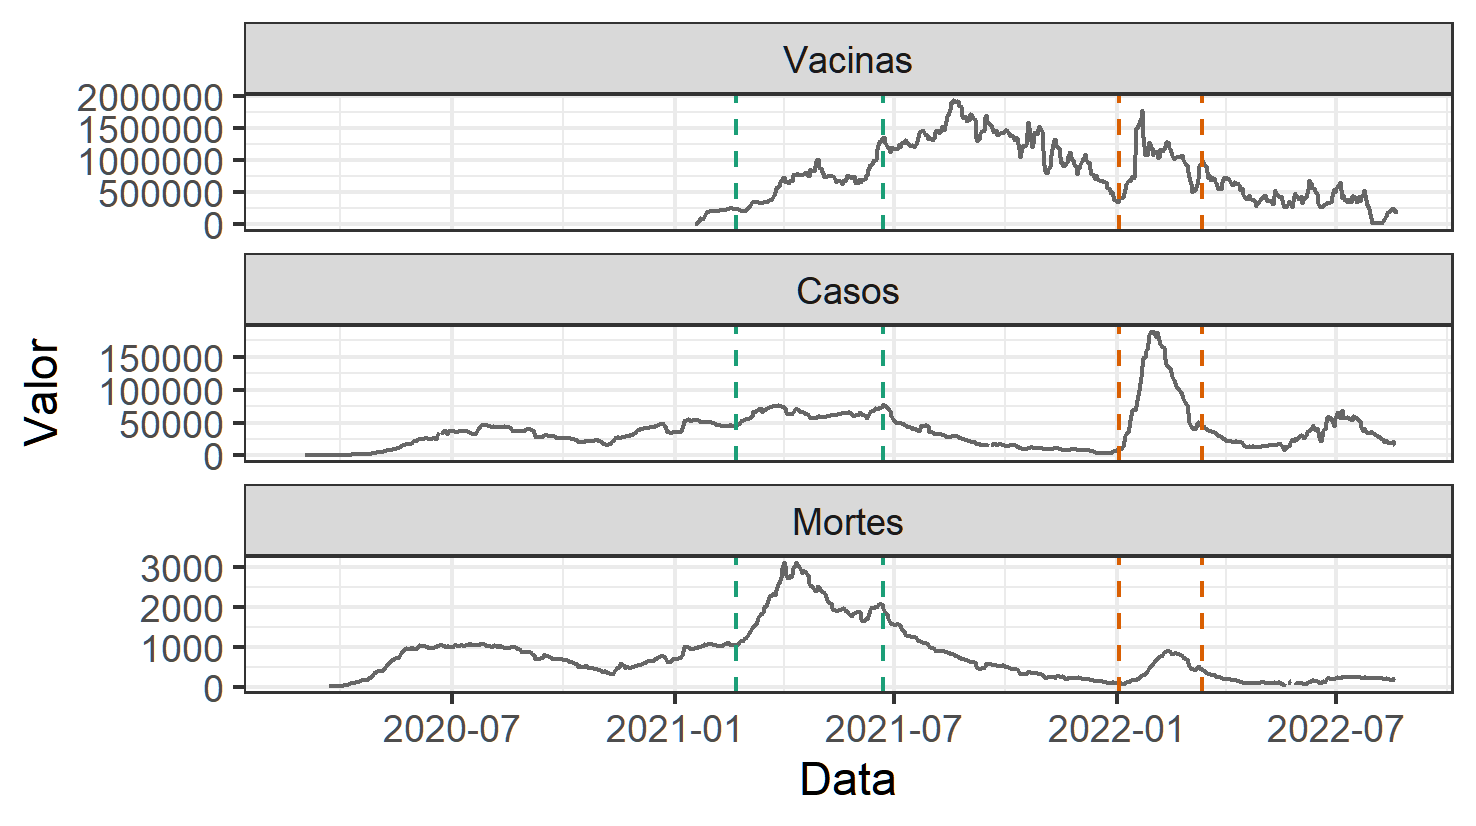
\includegraphics[]{Figuras/histval.png} %width = 0.84\textwidth
    \label{fig:histval}
\end{figure}

Porém, os dados de distanciamento disponíveis para o Brasil, porém, são de \textit{surveys} de preenchimento voluntário e individual (sem um entrevistador), que podem apresentar dados viesados, não representam a população brasileira como um todo, e estão disponíveis para uma janela de dados bem pequena. A falta desses dados afeta principalmente o método da IRF de vacinas em casos/mortes, já que o viés de variável omitida dificulta a interpretação causal dessa função. Como explicado na seção anterior, parte da dinâmica do distanciamento é explicada pelas próprias variáveis do sistema, de modo que a falta dos dados não prejudica os resultados tão intensamente.

A figura \ref{fig:acfall} apresenta as autocorrelações (padrões, parciais, e cruzadas) das séries. As variáveis têm muitos \textit{lags} significativos em suas ACF's, e apenas o primeiro em suas PACF's, indicando que os processos são auto-regresivos e médias-móveis. Vemos que a dependência do passado começa positiva, mas em \textit{lags} da casa das centenas o efeito se reverte. Além disso, casos parecem depender de seu passado mais fracamente que casos e vacinas.

As CCF's mostram resultados intuitivos: \textit{lags} de casos estão correlacionados positivamente com mortes, e o contrário não é tão significativo; \textit{Lags} de vacinas estão correlacionados negativamente com casos e mortes (em um primeiro momento), algo provavelmente relacionado efeitos da vacina; E o número de vacinas aplicadas parece se relacionar positivamente ao número passado de casos e mortes, algo passível de ser interpretado como a resposta de produtores, governos, e ``tomadores de vacinas'' à um aumento de casos.

\begin{figure}[H]
    \centering
    \caption{Autocorrelações das séries}
    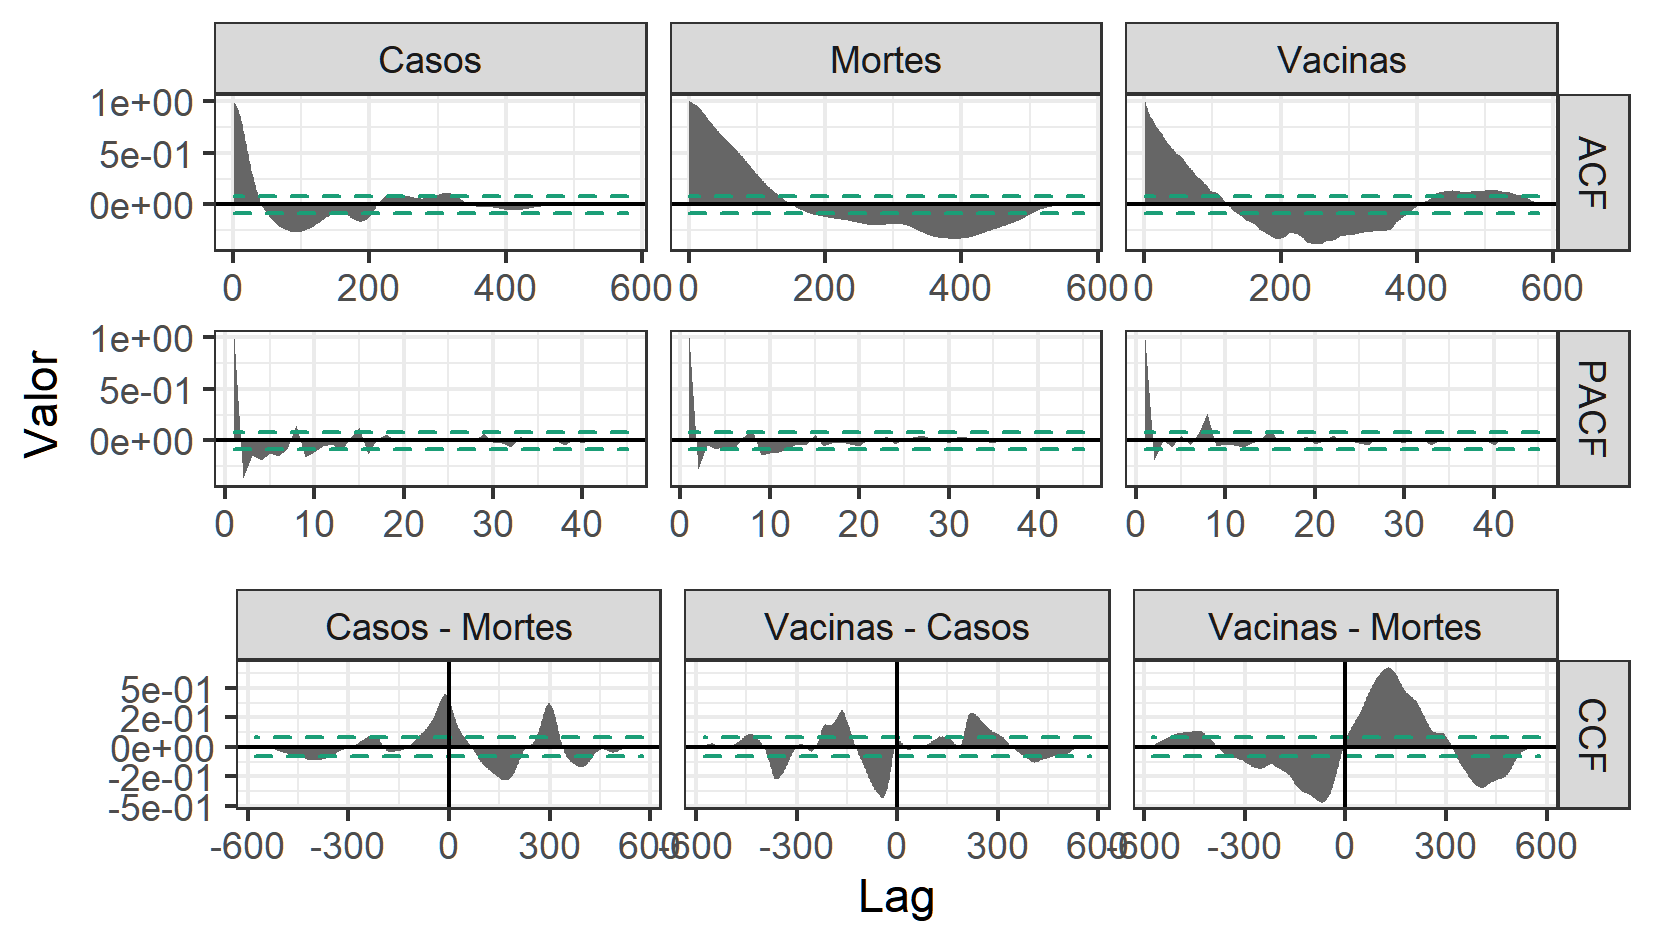
\includegraphics[width = 0.84\textwidth]{Figuras/acfall.png}
    \label{fig:acfall}
\end{figure}

Uma análise das correlações cruzadas antes e depois da vacinação já indica o possível efeito dessa variável, a correlação entre \textit{lags} de casos e mortes é maior no período pré vacina, como mostra a figura \ref{fig:ccfad}, indicando um aumento na resistência contra a doença na população pós vacina. Essa diferença é ainda maior no cenário da política de vacinação mais avançada como, por exemplo, 3 meses pós vacina.

\begin{figure}[H]
    \centering
    \caption{CCF's de casos e mortes, antes e depois da vacina}
    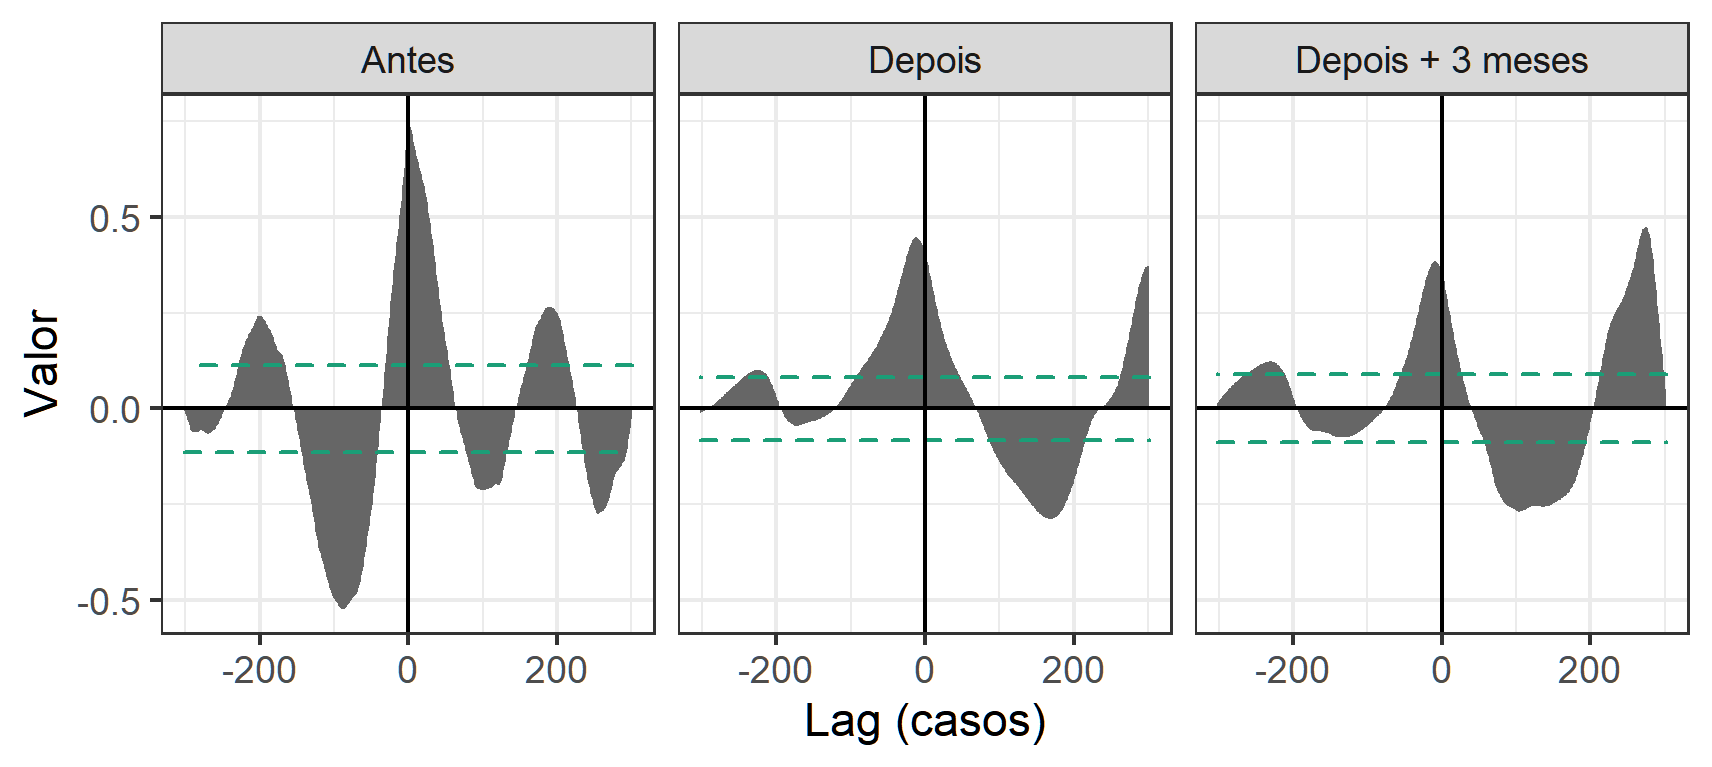
\includegraphics[]{Figuras/ccfad.png} %width = 0.84\textwidth
    \label{fig:ccfad}
\end{figure}



\let\clearpage\relax
\chapter{Modelo Econométrico}\label{sec:model}

Para realizar as três abordagens diferentes citadas na seção do modelo teórico, foram estimados dois VAR's:

\begin{align}
&\begin{bmatrix}
I_t \\ D_t
\end{bmatrix}
= \alpha_0^1 + \sum_{j=1}^{J^1}\pmb{\phi}_j^1
\begin{bmatrix}
I_{t-j} \\ D_{t-j}
\end{bmatrix}
+ \pmb{\alpha}^1_1m\hat{e}s_t + \pmb{\alpha}^1_2onda_t + \pmb{\varepsilon}_{t}^1, \;\; t \in \{0, 1, ..., t_v\} \label{eq:var1}\\
&\text{Modelo (1) estimado na amostra } t \in \{t_v, t_v+1, ..., t_f\}\label{eq:var2}\\
&\begin{bmatrix}
I_t \\ V_t \\ D_t
\end{bmatrix}
= \alpha_0^3 + \sum_{j=1}^{J^2}\pmb{\phi}_j^3
\begin{bmatrix}
I_{t-j} \\ V_{t-j} \\ D_{t-j}
\end{bmatrix}
+ \pmb{\alpha}^3_1m\hat{e}s_t + \pmb{\alpha}^3_2onda_t + \pmb{\varepsilon}_{t}^3, \;\; t \in \{t_v, t_v+1, ..., t_f\}\label{eq:var3}
\end{align}

\noindent Onde $t_v$ é a data da primeira vacina e $t_f$ é a última data na base de dados. $V_t$ é o número de vacinas aplicadas no período $t$, $I_t$ é o número de casos registrados no período, e  $D_t$ é o número de mortes registrados no período. $onda_t$ é um vetor de \textit{dummies} de primeira e segunda onda (como definidas pela figura \ref{fig:histval}), e $m\hat{e}s_t$ é um vetor de \textit{dummies} de mês do ano.

O modelo \eqref{eq:var1} é o modelo pré vacinação, \eqref{eq:var3} o modelo pós vacinação, e \eqref{eq:var2} um modelo ``intermediário''. Ele já apresenta a nova dinâmica entre casos e mortes pós vacinas, mas não leva em conta o efeito ``indireto" dessas variáveis com vacinas, por isso, a princípio, deve apresentar os efeitos positivos da vacinação, mas em menor intensidade do que o segundo \eqref{eq:var3}.

As \textit{dummies} de sazonalidade foram incluídas para capturar efeitos associados aos meses como variações de temperatura\footnote{\cite{Qi2020} mostra uma relação entre temperatura e umidade na transmissão do COVID-19 na China.}, e relaxamento do distanciamento social durante meio e fim de ano. Foram testadas outras \textit{dummies}, como mês e ano (mar. de 2020 a set. de 2022), semana no ano (de 0 a 52), e ordem da semana no mês (1 a 4). Porém nenhuma delas gerou grandes mudanças na captura da dinâmica das variáveis, e portanto, foi escolhido o modelo mais parsimonioso.

A seleção do número de \textit{lags} $J$ para cada modelo, foi feita com base no critério Akaike. Do primeiro ao último, o \textit{lag} escolhido foi $J^1 = 1$, $J^2=2$, e $J^3=3$. Todos os modelos foram estimados por MQO equação-a-equação. Os diagnósticos dos três modelos são similares, e os testes para o modelo \eqref{eq:var3} são apresentados no apêndice \ref{ap:diag}.

Em seguida os efeitos contemporâneos entre as variáveis foram modelados utilizando a decomposição de Cholesky. Foi feita a decomposição na ordem casos-vacinas-mortes, gerando a seguinte matrizes de relações contemporâneas:

\begin{equation}\label{eq:svar}
    \begin{bmatrix}
    \varphi_{II}^1 & 0 & 0 \\
    \varphi_{IV}^1 & \varphi_{VV}^1 & 0 \\
    \varphi_{ID}^1 & \varphi_{VD}^1 & \varphi_{DD}^1
    \end{bmatrix}
\end{equation}


Todo o trabalho computacional foi realizado utilizando o \textit{software} R e o pacote \textit{vars}\footnote{O repositório de github com o código outras informações pode ser encontrado \href{https://github.com/ricardo-semiao/TCC-Graduacao}{neste link}.}.

\let\clearpage\relax
\chapter{Resultados e discussão}

A seção \ref{sec:res1} calcula as IRF's dos três modelos VAR, utilizando a decomposição em \eqref{eq:svar}, mostrando como a inclusão de vacinas afeta as funções. A seção \ref{sec:res2} constrói contrafactuais da não existência de vacinas com vários métodos diferentes, obtendo estimativas do efeito total da política de vacinação.

Antes de apresentar os resultados principais, vale a pena mostrar como correlação entre $\hat{\varepsilon}^i_{Casos}$ e $\hat{\varepsilon}^i_{Mortes}$\footnote{$\hat{\varepsilon}^i$ indica vetor de resíduos do modelo (i).} diminuiu após o início da vacinação. Nos três modelos VAR, respectivamente: $\mathbb{COR}(\hat{\varepsilon}^i_{Mortes}, \hat{\varepsilon}^i_{Casos}) = 0,908$, $0,405$, e $0,373$. Esse fato é uma evidência preliminar sobre como a vacina imunizou a população a um choque de casos.

\section{Resposta de Mortes à Casos antes e Depois da Vacinação}\label{sec:res1}
O resultado principal deste trabalho é mostrar a diferença do impacto de um choque de casos pré e pós vacinação, algo que fica claro na figura \ref{fig:IRF BaA}, que mostra a resposta de mortes após um choque de 1000 casos\footnote{Intervalos de confiança de 90\%, calculados por \textit{bootstrap}.}, para o SVAR identificado na ordem casos-vacinas-mortes.

\begin{figure}[H]
    \centering
    \caption{IRF's de Casos em Mortes Antes e Depois da Vacinação}
    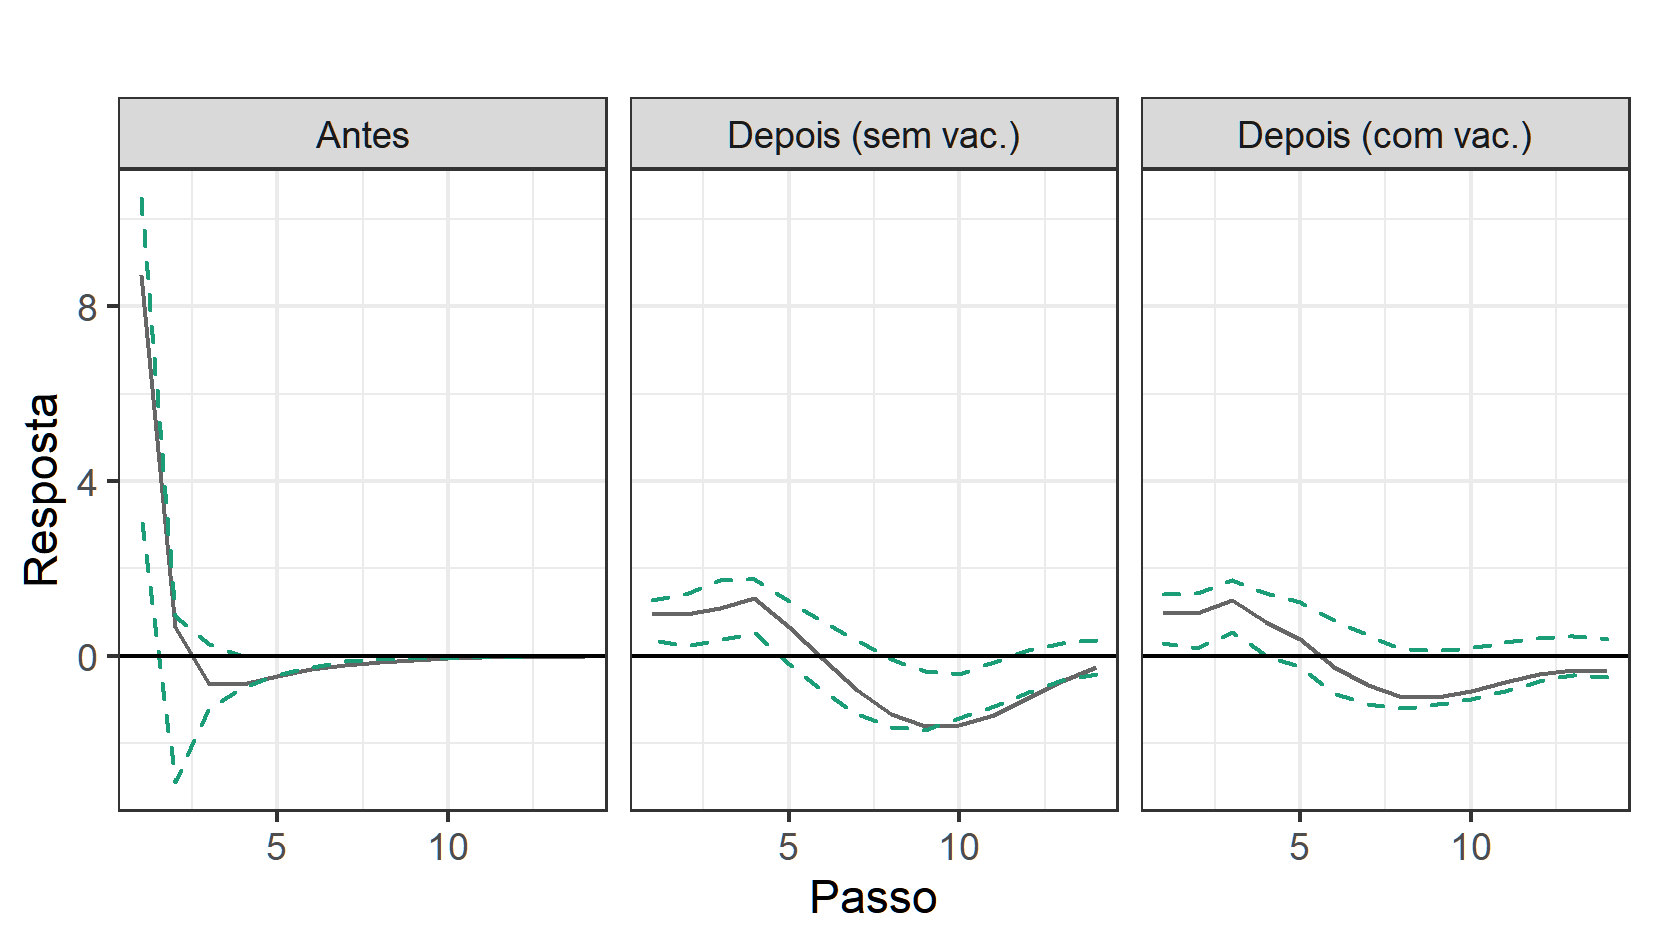
\includegraphics[width = 0.95\textwidth]{Figuras/IRF BaA CVM.png}
    \label{fig:IRF BaA}
\end{figure}

Antes da vacinação, um choque de $1000$ casos gerava $8,71$ mortes na primeira semana, e depois se estabilizava em torno do 0 a partir da segunda/terceira semana. Depois da vacinação, o modelo sem vacinas apresenta uma resposta de $1,33$ mortes na primeira semana, e também se estabiliza para valores insignificantes em seguida (por mais que a estabilização demora mais). No modelo \eqref{eq:var3}, que leva em conta o efeito que casos e mortes tem na provisão de vacinas, a IRF fica ainda menor, apresentando um pico de $1,28$ mortes. Esses resultados podem ser vistos na tabela \ref{tb:irfpico}.

\begin{table}[H]
\centering
\caption{Variações no Pico das IRF's}
\label{tb:irfpico}
\begin{tabular}{ccccc}
\\[-1.8ex]\hline 
\hline \\[-1.8ex] 
Modelo & Estimativa & IC (95\%) & IC (90\%) & IC (68\%) \\\hline\\[-1.8ex]
\multicolumn{1}{c|}{\eqref{eq:var1}}                   & 8.71 & 2.21 a 10.35 & 3.14 a 10.69 & 3.83 a 9.05 \\ 
\multicolumn{1}{c|}{\eqref{eq:var2}}                   & 1.33 & 0.16 a 1.86 & 0.13  a 1.79 & 0.07  a 1.47 \\ 
\multicolumn{1}{c|}{\eqref{eq:var3}}                   & 1.28 & 0.11 a 1.74 & 0.09  a 1.78 & 0.16  a 1.8 \\ 
\multicolumn{1}{c|}{}                                  &  &  &  &  \\ 
\multicolumn{1}{c|}{\eqref{eq:var1} - \eqref{eq:var3}} & 7.43 & 0.47 a 10.24 & 1.36 a 10.6 & 2.03 a 8.89 \\ 
\multicolumn{1}{c|}{Proporção}                         & 85\% & 21\% a 99\% & 43\%  a 99\% & 53\%  a 98\% \\ 
\\[-1.8ex]\hline 
\hline \\[-1.8ex] 
\end{tabular}
\end{table}

Só o pico não passa toda a mudança de dinâmica, a vacinação pode afetar também a trajetória das funções. A vacinação pode fazer com que o tempo de cama antes do falecimento aumente, ``atrasando'' a resposta. Além disso, a vacinação pode deixar a população mais confiante, diminuindo a resposta no distanciamento dado um choque de casos. Por outro lado, mesmo com menos distanciamento, a menor taxa de mortalidade reduz o aumento de mortes dado um menor distanciamento. Em suma, não é óbvio se a trajetória da IRF muda, ou se se mantém similar, apenas em menor escala.

Por esse motivo, vale também analisar as mudanças nas somas dos valores das funções (tabela \ref{tb:irfsoma}). A soma da resposta à $1000$ casos é de $22,62$ mortes, reduzindo para $5.04$ no modelo intermediário, e $4,41$ no último modelo, representando uma diminuição na resposta de $18,21$ mortes (ou 81\%). Em proporção, os valores são similares.

\begin{table}[H]
\centering
\caption{Variações na Soma das IRF's}
\label{tb:irfsoma}
\begin{tabular}{ccccc}
\\[-1.8ex]\hline 
\hline \\[-1.8ex] 
Modelo & Estimativa & IC (95\%) & IC (90\%) & IC (68\%) \\\hline\\[-1.8ex]
\multicolumn{1}{c|}{\eqref{eq:var1}}                    & 22.62 & 3.22 a 28.73 & 3.35 a 24.68 & 5.57 a 20.74 \\ 
\multicolumn{1}{c|}{\eqref{eq:var2}}                    & 5.04 & 1.34  a 8.28 & 0.97  a 7.21 & 2.31  a 5.96 \\ 
\multicolumn{1}{c|}{\eqref{eq:var3}}                    & 4.41 & 0.81  a 7.76 & 1.02  a 8.19 & 1.3   a 7.71 \\ 
\multicolumn{1}{c|}{}                                   &  &  &  &  \\ 
\multicolumn{1}{c|}{\eqref{eq:var1} - \eqref{eq:var3}}  & 18.21 & -4.54 a 27.92 & -4.84 a 23.66 & -2.14 a 19.44 \\ 
\multicolumn{1}{c|}{Proporção}                          & 81\% & -141\% a 97\% & -144\% a 96\% & -38\% - 94\% \\ 
\\[-1.8ex]\hline 
\hline \\[-1.8ex] 
\end{tabular}
\end{table}

Por último, note que estamos interpretando a IRF sem vacina como um contrafactual da ``IRF no período pós vacinas, mas no mundo onde a vacinação não ocorreu''\footnote{A princípio essa interpretação faz sentido, como discutido no final da seção \ref{sec:teorico2}}. Com isso em mente, podemos extrapolar os resultados dessa seção, e multiplicar a soma da IRF pós vacinas pelo total de casos (dividido por mil, uma vez que essa era o tamanho do choque). Os resultados desse método são apresentados no fim da seção seguinte.

Na hora de interpretar os resultados dessa metodologia, é importante ter em mente que as IRF's analisadas são uma aproximação linear das respostas durante o período analisado, sem permitir variações nessas funções com base nos níveis das outras variáveis, algo que o modelo SIRDV assumia ser importante. Se, por exemplo, a resposta à vacinas cai muito conforme o número de imunizados sobe, essa metodologia deve apresentar um resultado muito superestimado.


\section{Análise de Contrafactual}\label{sec:res2}
Para ter uma medida do efeito total da política de vacinação, é possível construir um contrafactual onde nunca houve a vacinação, e comparar com os casos e mortes observados. Para isso, foram elencados alguns métodos diferentes: (i) utilizar o modelo \eqref{eq:var1} para ``prever'' o período pós vacinas; (ii) utilizar o modelo \eqref{eq:var3} e calcular a série de casos e mortes, dado o ponto inicial pré vacinas, e forçando a equação de vacinas a ser zero (zerando também a influência dela sobre casos e mortes); (iii) e (iv) envolvem as mesmas duas abordagens anteriores, mas em vez de calcular a variável de casos com o modelo, utilizar a variável de casos observada para calcular um contrafactual apenas para mortes.


Os contrafactuais de cada abordagem são ligeiramente diferentes: (iii) e (iv) estimam ``qual seria o número de mortes no 'mundo' sem vacinas, mas onde os casos se mantiveram iguais?''; enquanto (i) e (ii) estimam ``qual seria o número de mortes no mundo sem vacinas, dado que a falta de vacinas (possivelmente) também afetaria o número de casos''. Embora a abordagem (i) e (ii) parece ser o contrafactual mais ``completo'', não isolam o efeito da redução de mortalidade. Como o efeito da vacina na taxa de infecção e número de casos não é tão claro, os contrafactuais (i) e (ii) são de mais difícil interpretação. Nesse sentido, (iii) parece ser o modelo mais promissor.

As abordagens (ii) e (iv) incluem a mudança da relação entre casos e mortes pós vacinas, em sua estimação, apenas ``zerando'' o efeito direto da vacina, portanto devem apresentar um contrafactual mais conservador. Ao mesmo tempo, devem ser mais precisos, uma vez que, o modelo \eqref{eq:var3} foi estimado com o dobro de observações do \eqref{eq:var1}. Lembrando que todas as \textit{dummies} de mês e onda foram utilizadas nas ``previsões''.

\begin{figure}[H]
    \centering
    \caption{Contrafactuais (i) e (ii)}
    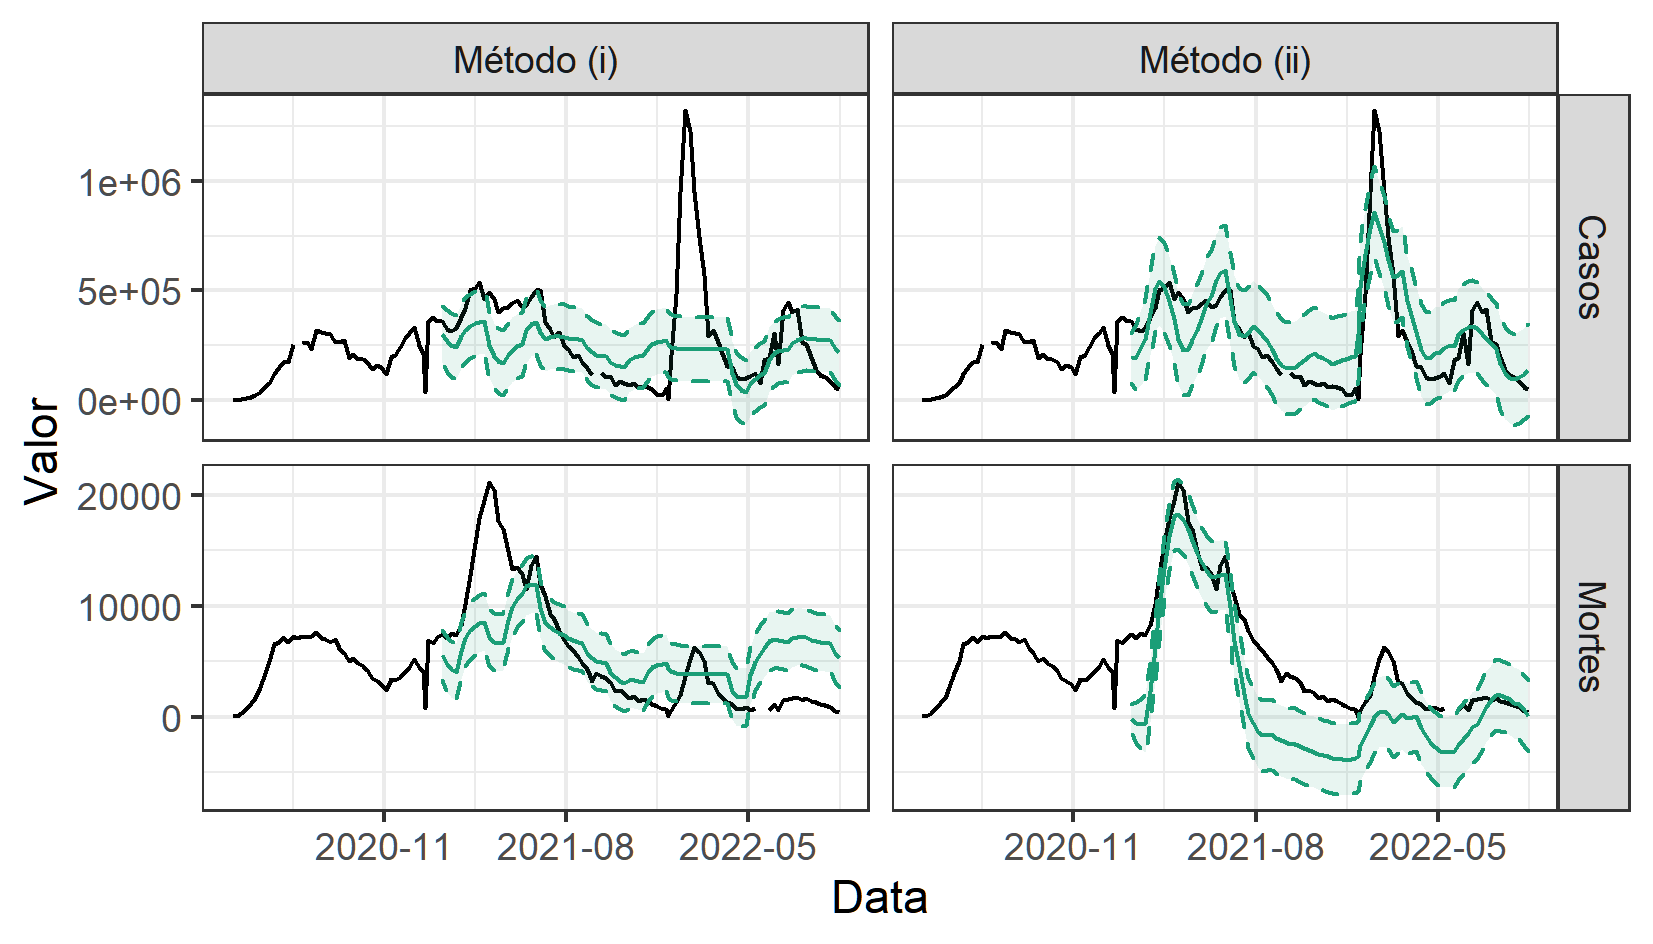
\includegraphics[width = 0.95\textwidth]{Figuras/counterfactual.png}
    \label{fig:counter1}
\end{figure}

Os resultados dos métodos (i) e (ii) podem ser vistos na figura \ref{fig:counter1}. A figura apresenta o intervalo de confiança de 95\%. Como esperado, o método (ii) segue as séries realizadas com muito mais precisão, inclusive ``prevendo'' a segunda onda de casos. Porém, ambas as metodologias mostram um número reduzido de casos, o que dificulta a interpretação do efeito da redução da mortalidade.

Os resultados dos métodos (iii) e (iv) podem ser vistos na figura \ref{fig:counter2}. O problema do método (ii) é intensificado com a inclusão dos casos realizados, e (iv) apresenta um contrafactual basicamente idêntico à série realizada. O método (iii) apresenta uma mortalidade bem maior na primeira onda (em comparação à (i)), mas não responde rapidamente à segunda onda de casos, gerando, novamente, um contrafactual com menos mortes.

\begin{figure}[H]
    \centering
    \caption{Contrafactuais (iii) e (iv)}
    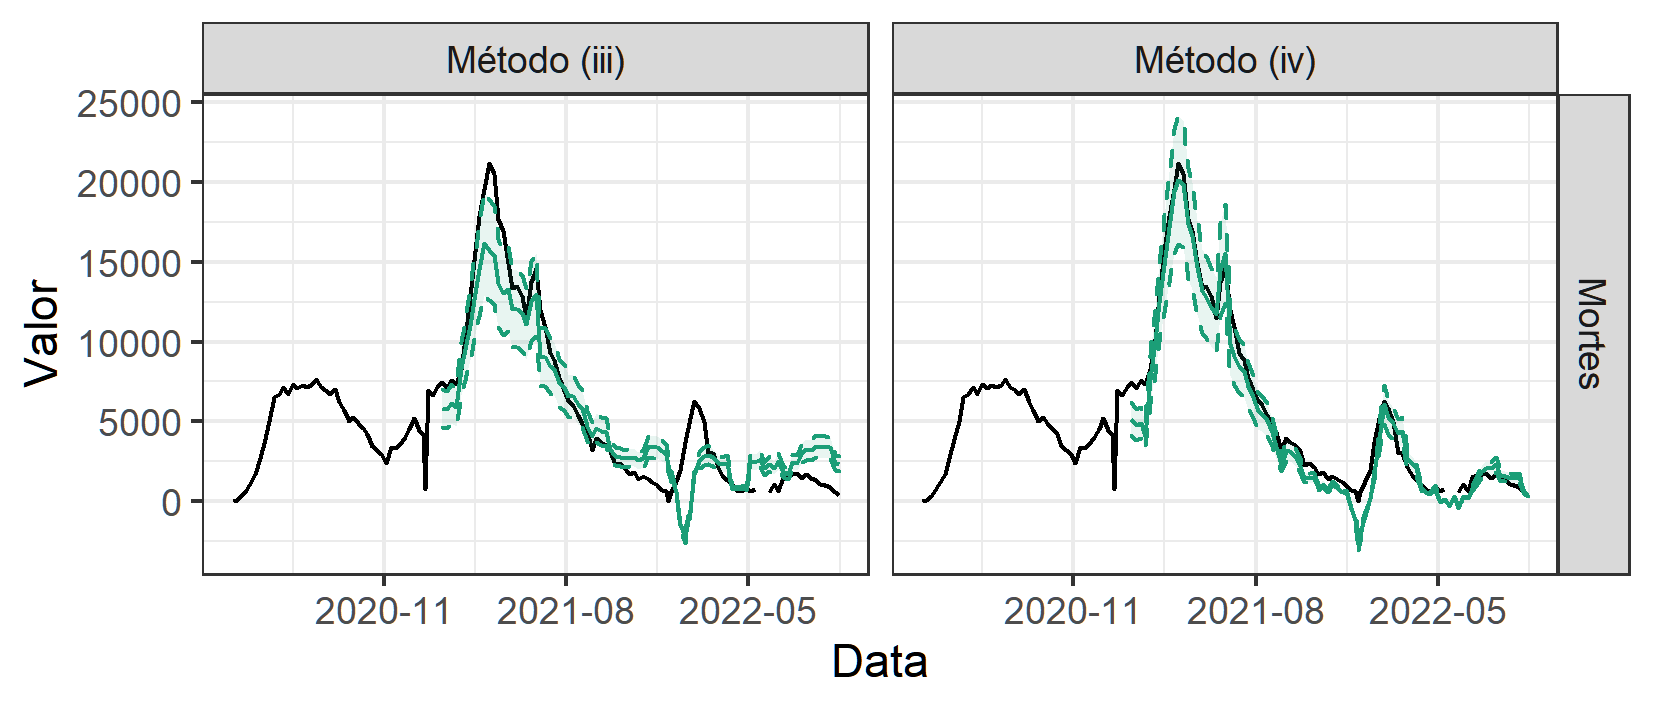
\includegraphics[width = 0.95\textwidth]{Figuras/counterfactual2.png}
    \label{fig:counter2}
\end{figure}

O resultado de todos os modelos pode ser encontrado no apêndice \ref{ap:count}. Como discutido anteriormente, os métodos (ii) e (iv) retornaram um número de mortes pequeno, inclusive menor que o valor real, portanto, a análise será focada nos contrafactuais mais ``completos'' (i) e (iii).

Como a comparação do pico das IRF's não levam em conta as alterações que a vacinação faz na trajetória (advindas de mudanças no distanciamento, tempo de cama, entre outros), podemos comparará-las com às IRF's soma para entender a importância relativa de cada efeito. Para serem comparáveis às metogias dessa seção, o número total de casos escolhido para multiplicar as IRF's foi o valor estimado na metodologia (i). As comparações podem ser encontradas na tabela \label{tb:counter1}. Vemos que o efeito associado à IRF pico é apenas 40\% daquele associado à IRF soma, mostrando a importância da alteração das trajetórias das IRF's que a vacina gera.

\begin{table}[H] \centering 
\renewcommand{\arraystretch}{1.2}
  \caption{IRF Pico v.s. Soma)}\label{tb:counter1} 
\begin{tabular}{@{\extracolsep{5pt}} llccc} 
\\[-1.8ex]\hline 
\hline \\[-1.8ex] 
Método & Série & Diferença & Int. inferior & Int. superior \\ 
\hline \\[-1.8ex] 
IRF pico                   & Mortes    & 114.691       & 7.254         & 158.067 \\
IRF soma                   & Mortes    & 281.094    & -70.080       & 430.981 \\
\\[-1.8ex]\hline 
\hline \\[-1.8ex] 
\end{tabular} 
\end{table} 

A tabela \ref{tb:counter2} apresenta os modelos (i) e (ii) (``VAR antes'' e ``VAR antes *''), bem como a ``IRF soma'', e a IRF soma mas calculada com o valor real da variável de casos, ``IRF soma *''. Vemos que O método (i) ficou ligeiramente acima do método (iii), indicando que o efeito de vacinas em casos contribui com a redução de mortes no contrafactual. Dessa leva de métodos, (i) foi o único a retornar um contrafactual com menos mortes, e de acordo com essa metodologia, aprox. 31mil vidas foram salvas com a política de vacinação até set/2020\footnote{Um valor substancialmente menor do que aquele calculado por \cite{Ferreira2021}.}. Os métodos de IRF, geraram valores bem mais altos, possivelmente por, como discutido anteriormente, serem feitos com base em uma aproximação linear. A IRF soma calculada com os casos estimados, porém, pode ser considerada um \textit{upper bound} do efeito contrafactual.

\begin{table}[H] \centering 
\renewcommand{\arraystretch}{1.2}
  \caption{Análise de Contrafactual}\label{tb:counter2}
\begin{tabular}{@{\extracolsep{5pt}} llccc} 
\\[-1.8ex]\hline 
\hline \\[-1.8ex] 
Método & Série & Diferença & Int. inferior & Int. superior \\ 
\hline \\[-1.8ex] 
\multirow{2}{*}{VAR antes}  & Casos     & -8.007.319    & -17.294.129   & 2.512.505 \\ 
                            & Mortes    & 31.153        & -184.661      & 249.452 \\ 
VAR antes *                 & Mortes    & -16.403       & -106.588      & 73.782  \\ 
\\[-1.8ex] 
IRF soma                   & Mortes    & 281.094    & -70.080       & 430.981 \\
IRF soma *                  & Mortes    & 467.088       & -116.451        & 716.150 \\
\\[-1.8ex]\hline 
\hline \\[-1.8ex] 
Obs: & \multicolumn{4}{r}{''*'': estimado com o valor de casos real}
\end{tabular} 
\end{table} 


\let\clearpage\relax
\chapter{Conclusão}
Nesta tese, foram desenvolvidas diferentes abordagens para medir medido efeito das vacinas no número de casos mortes que o Brasil apresentou durante a pandemia do COVID-19.

Motivado pela natureza de dinâmica temporal entre as variáveis, como explicada no modelo teórico SIRDV, foi realizada uma modelagem SVAR, incomum na literatura epidemiológica. A identificação do modelo também foi feita consistentemente com a teoria.

A abordagem mais robusta comparou as IRF's de SVAR'es estimados antes e depois do início da vacinação, controlando possíveis falhas na especificação do modelo ao analisar como a vacina o altera. Essa abordagem mostrou a variação na soma da resposta em mortes, dado um choque de 1000 casos, é de 18.21 em termos absolutos, e 81\% em termos proporcionais. Isto é, a taxa de mortalidade de um choque de casos foi diminuída drasticamente após o início da política de vacinação, mostrando o quão eficaz esta foi.

A outra abordagem foi a criação de um contrafactual para estimar o efeito agregado da vacinação. Foi identificado um \textit{lower} e um \textit{upper bound} de, respectivamente 31mil e 281mil vidas salvas até set/2020, sendo que o segundo apresenta indícios de superestimação, mas é mais consistente com a redução forte das IRF's discutida acima.

Esta tese apresentou mais uma metodologia para atestar a eficiência da vacinação, servindo como mais um insumo para a busca de um consenso na literatura e fim da desinformação, além de ser mais uma ferramenta para os \textit{policymakers} definirem o gasto e urgência ótima para as políticas de vacinação. Além disso, é a primeira que utiliza uma metodologia SVAR para a pandemia do COVID-19, e mostrou que existe a capacidade de obter resultados mais informativos que apenas o efeito agregado da vacinação.

O potencial da metodologia não foi explorado até o fim, existe espaço para a busca de novas técnicas de identificação, busca de dados de melhor qualidade, e inclusão do distanciamento social nos modelos. Com isso seria possível aprimorar as estimativas obtidas, e tornar possível analisar as IRF's de vacinas em mortes e casos, gerando um resultado de efeito marginal muito útil. Similarmente, existe muito espaço para aplicações dessa metodologia em outros contextos para evidenciar seu bom funcionamento.



% ----------------------------------------------------------
% ELEMENTOS PÓS-TEXTUAIS
% ----------------------------------------------------------
\postextual

% ---
% Referências bibliográficas
\newpage
\printbibliography
% ---

% ---
% Apêndices
\newpage
\begin{apendicesenv}
\chapter{Resultados da Análise de Contrafactual}\label{ap:count}
\begin{table}[H] \centering 
\renewcommand{\arraystretch}{1.2}
  \caption{Diferença do Contrafactual e do Realizado}\label{tb:counter} 
\begin{tabular}{@{\extracolsep{5pt}} llccc} 
\\[-1.8ex]\hline 
\hline \\[-1.8ex] 
Método & Série & Diferença & Int. inferior & Int. superior \\ 
\hline \\[-1.8ex] 
\multirow{2}{*}{VAR antes}  & Casos     & -8.007.319    & -17.294.129   & 2.512.505 \\ 
                            & Mortes    & 31.153        & -184.661      & 249.452 \\ 
\multirow{2}{*}{VAR depois} & Casos     & -1.389.775    & -15.044.853   & 19.651.972 \\ 
                            & Mortes    & -201.148      & -279.654      & -27.897 \\
\\[-1.8ex] 
VAR antes *                 & Mortes    & -16.403       & -106.588      & 73.782  \\ 
VAR depois *                & Mortes    & -40.882       & -126.171      & 44.408  \\ 
\\
IRF pico                    & Mortes    & 114.691       & 7.254         & 158.067 \\
IRF soma                    & Mortes    & 281.094       & -70.080       & 430.981 \\
\\[-1.8ex] 
IRF pico *                  & Mortes    & 190.580       & 12.055        & 262.656 \\
IRF soma *                  & Mortes    & 467.088       & -116.451        & 716.150 \\
\\[-1.8ex]\hline 
\hline \\[-1.8ex] 
Obs: & \multicolumn{4}{r}{''*'': estimado com o valor de casos real}
\end{tabular} 
\end{table} 


\chapter{Diagnósticos do VAR}\label{ap:diag}
Antes de sua inclusão no VAR \eqref{eq:var3}, foi realizado um teste de raiz unitária sobre as séries, apresentado na tabela \ref{tb:testadf}. Podemos ver que apenas nenhuma série é estacionária.

\begin{table}[H] \centering 
  \caption{Teste Dickey-Fuller Aumentado} 
  \label{tb:testadf} 
\begin{tabular}{@{\extracolsep{5pt}} ccccc} 
\\[-1.8ex]\hline 
\hline \\[-1.8ex] 
 & Variável & Estatística & Lag & P-valor \\ 
\hline \\[-1.8ex] 
1 & Vacinas & -2.78 & 4 & 0.26 \\ 
2 & Casos & -2.36 & 4 & 0.43 \\ 
3 & Mortes & -2.66 & 4 & 0.30 \\ 
\hline \\[-1.8ex] 
\end{tabular} 
\end{table} 

A comparação do fit do modelo VAR e os valores reais, bem como o resíduo resultante, está presente na figura \ref{fig:varfit}. A distribuição dos resíduos parece relativamente ter uma volatilidade similar ao longo da reta de valores fitados, e de fato, o teste ARCH-LM não indicou a presença de erros ARCH no modelo -- estatística do teste de $206.61$, com $180$ graus de liberdade, gerando um p-valor $< 0.0848$.

\begin{figure}[H]
    \centering
    \caption{Fit do VAR}
    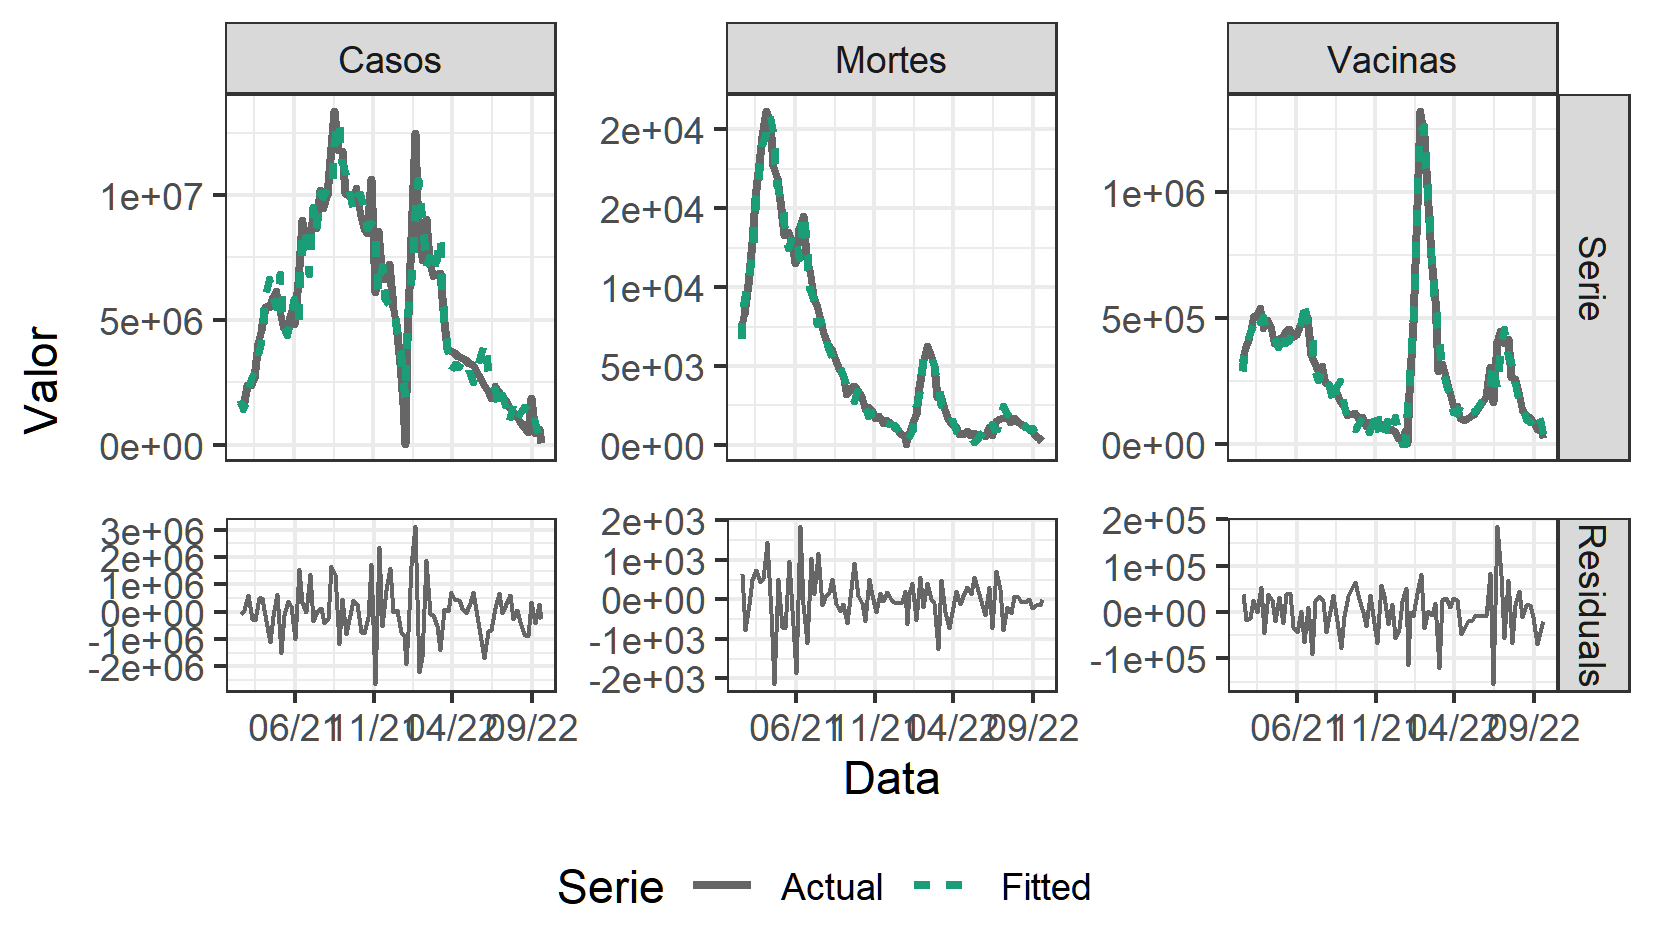
\includegraphics[width = 0.84\textwidth]{Figuras/varfit.png}
    \label{fig:varfit}
\end{figure}

Podemos ver mais detalhes dos resíduos na figura \ref{fig:varresdist}, que mostra uma variância dos resíduos não tão dependente dos valores do modelo, mas uma distribuição não exatamente normal. Realmente, o teste Jarque-Bera multivariado indica erros não normais -- estatística do teste de $42.113$, com 6 graus de liberdade, gerando um p-valor de $1.747e-07$. Embora isso comprometa em alguma medida os testes de hipótese, principalmente do teste de causalidade de Granger, esse resultado não é um grande problema.

\begin{figure}[H]
    \centering
    \caption{Distribuição dos resíduos do VAR}
    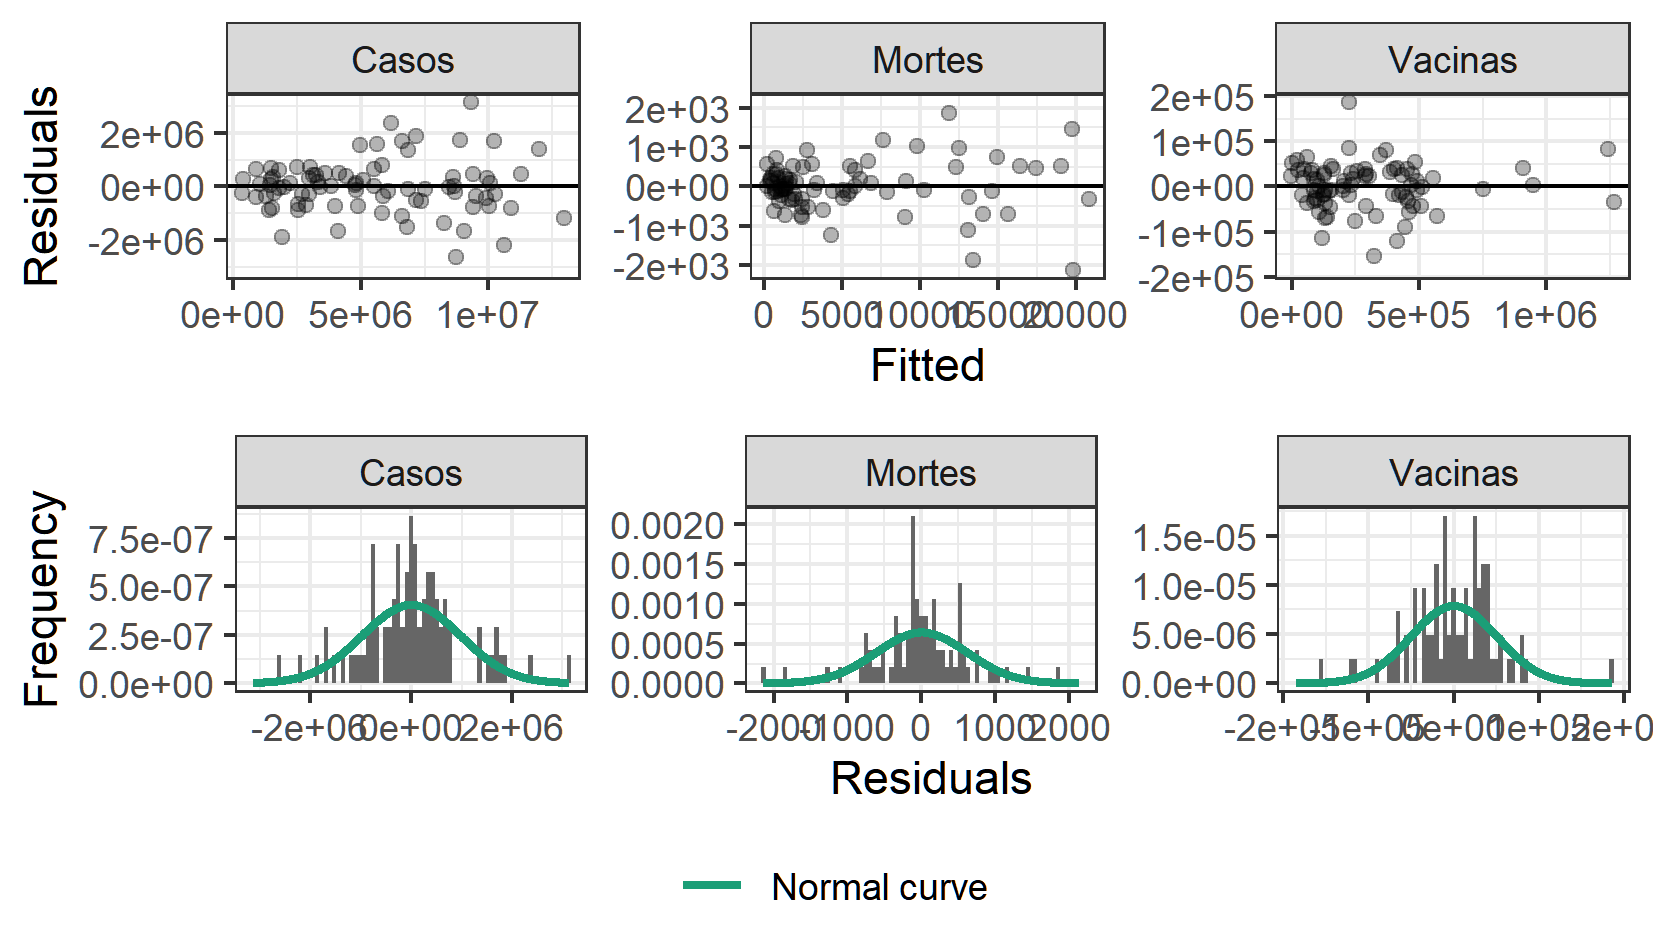
\includegraphics[]{Figuras/varresdist.png} %width = 0.84\textwidth
    \label{fig:varresdist}
\end{figure}

A figura \ref{fig:varresacf} mostra as autocorrelações dos resíduos, indicando dependência temporal insignificante das e entre as variáveis. De fato, o modelo passou teste Portmanteau de autocorrelação dos resíduos (em até 12 lags) -- estatística do teste de 123.54, com 117 graus de liberdade, gerando um p-valor = 0.3215. Similarmente, o teste Edgerton-Shukur também rejeitou a presença de autocorrelação.

\begin{figure}[H]
    \centering
    \caption{Autocorrelações dos resíduos do VAR}
    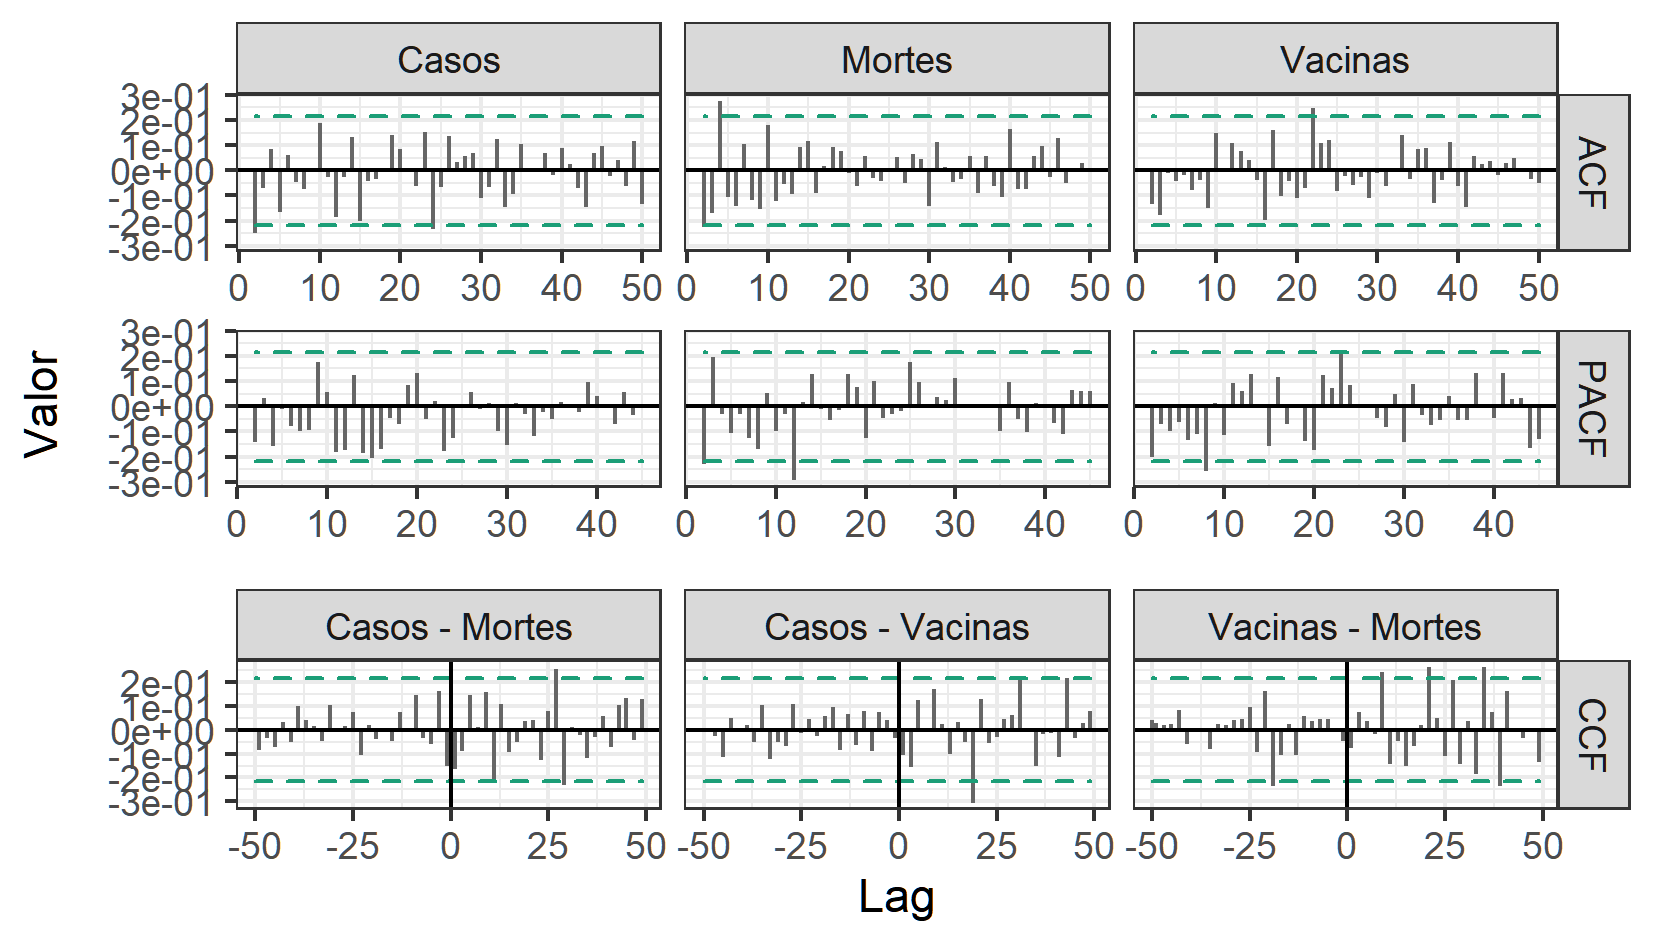
\includegraphics[]{Figuras/varresacf.png} %width = 0.84\textwidth
    \label{fig:varresacf}
\end{figure}

A figura \ref{fig:varstab} mostra o teste CUMSUM baseado nos resíduos das equações MQO, mais especificamente, é o resultado da função ``stability'' do pacote ``vars'' com o método ``CUMSUM-OLS'' no R. Ela indica que alterar a amostra que baseou a estimativa do modelo não altera drasticamente os valores dos coeficientes.

\begin{figure}[H]
    \centering
    \caption{Estabilidade do VAR}
    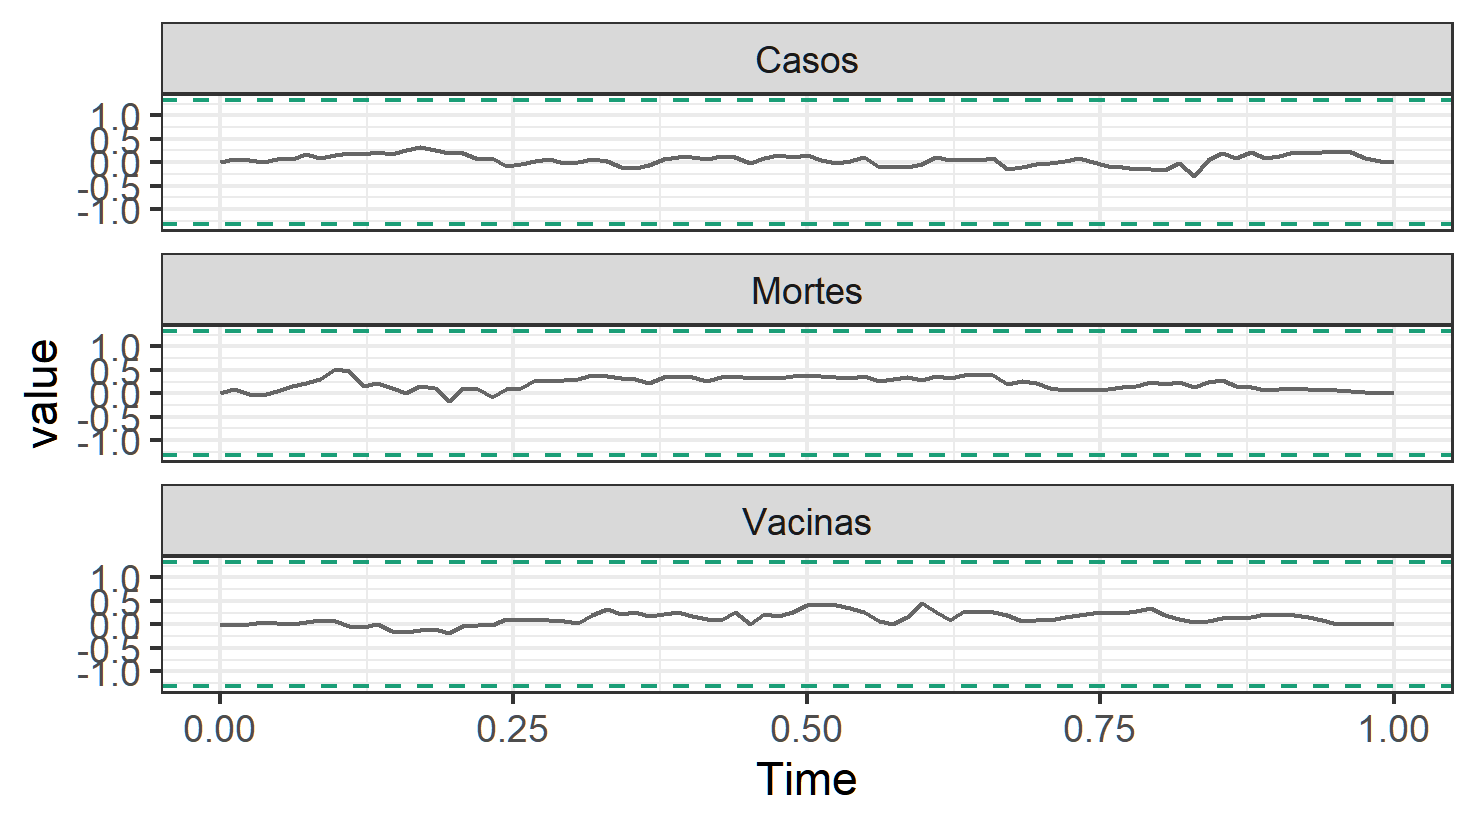
\includegraphics[]{Figuras/varstab.png}
    \label{fig:varstab}
\end{figure}

Vale atentar que as raízes do VAR são todas menores que 1: $0.909 (<1)$,	$0.886 (<1)$,	$0.886 (<1)$,	$0.754 (<1)$,	$0.754 (<1)$,	$0.563 (<1)$,	$0.563 (<1)$,	$0.522 (<1)$,	$0.522 (<1)$.

Por fim, o R quadrado de cada equação é: Casos 0.960, Vacinas 0.918, Mortes 0.988

\newpage

\end{apendicesenv}
% ---

\end{document}
